\documentclass[11pt, oneside]{book}
\usepackage[a4paper,width=135mm,top=30mm,bottom=30mm]{geometry}
%bindingoffset=12mm
\usepackage[utf8]{inputenc}
\usepackage{CJKutf8}  % Japanese support
\usepackage{setspace}

% mathematics notations
\usepackage{amsfonts}
\usepackage{amssymb}
\usepackage{amsmath}
\DeclareMathOperator{\argmin}{argmin}
\DeclareMathOperator{\argmax}{argmax}

% BibLaTex 
\usepackage[
	backend=biber,
	style=ieee,
	citestyle=ieee,
	natbib=false,
	url=false, 
	doi=false,
	arxiv=false,
	eprint=true,
	mincitenames=1
]{biblatex}
\addbibresource{../library.bib}

% Style
%%%%%%%%
%\setcounter{tocdepth}{0} % hide all subsection from table of content

% url, link
\usepackage{hyperref}
\hypersetup{
	colorlinks=true,
	linkcolor=cyan,
	filecolor=magenta,  
	citecolor=cyan,    
	urlcolor=blue,
}
\urlstyle{same}

% header and footer
\usepackage{fancyhdr}
\pagestyle{fancy}
\fancyhead{}
\fancyhead[L]{\leftmark}
\fancyhead[R]{\thepage}
\fancyfoot{}

% environment
%%%%%%%%

% enum
\usepackage{enumitem}
\setlist[description]{leftmargin=\parindent,labelindent=\parindent}
% algorithm
\usepackage{algorithm, algcompatible}
\usepackage[noend]{algpseudocode}
\renewcommand{\COMMENT}[2][.6\linewidth]{%
	\leavevmode\hfill\makebox[#1][l]{//~#2}}
\algnewcommand\RETURN{\State \textbf{return} }

% Draw
%%%%%%%%

\usepackage{tikz}
\usepackage{verbatim}
\usetikzlibrary{arrows,shapes}
\tikzstyle{vertex}=[node font=\footnotesize, fill=none,circle, draw, inner sep=2pt, minimum size = 14pt]
\tikzstyle{positive vertex}=[fill=none, circle, draw, text=blue, inner sep=0pt, minimum size = 14pt]
\tikzstyle{negative vertex}=[fill=none, circle, draw, text=red, inner sep=0pt, minimum size = 14pt]
\tikzstyle{edge} = [draw,line width=0.8pt,-]
\tikzstyle{thickedge} = [draw,line width=2pt,-]
\tikzstyle{dashedge} = [draw,thick, dashed]
\tikzstyle{note} = [draw=none, opacity=1, align=center]
\tikzstyle{synthetic data} = [minimum size = 5pt]

\usepackage{pgfplots}
\pgfplotsset{compat=1.5}
\pgfmathsetseed{10} 
\tikzstyle{positive data} = [only marks, mark=+, style=ultra thick, mark size=4, color=blue]
\tikzstyle{negative data} = [only marks, mark=-, style=ultra thick, mark size=4, color=red]
\tikzstyle{unlabeled data} = [only marks, mark=o, mark size=2]


% table
\usepackage{multirow}


\usepackage{caption}
\usepackage{subcaption}

\begin{document}
{
	\restoregeometry
	\begin{titlepage}
	\begin{center}
	\Large
	\vspace*{2cm}
	\begin{CJK}{UTF8}{min} 修士論文 \end{CJK}
	
	\vspace{1.5cm}
	
	\textbf{Study on Semi-Supervised Learning with\\ the Framework of Generative Model}
	
	\vspace{.3cm}
	
	\textbf{\begin{CJK}{UTF8}{min} 生成モデルを用いた半教師付き学習に関する研究 \end{CJK}}
	
	\vspace{2cm}
	
	\begin{CJK}{UTF8}{min} 2019年6月26日 \end{CJK}
	
	\vspace{2cm}
	
	\begin{CJK}{UTF8}{min} 学籍番号 \quad 17507781 \end{CJK}\\
	\vspace{.2cm}
	\textbf{NGUYEN HOANG NGHIA}
	
	\vspace{2cm}
	
	\begin{CJK}{UTF8}{min} 指導教員 \quad 山田 \enskip 耕一 \end{CJK}		
	
	\vspace{2cm}
	
	\begin{CJK}{UTF8}{min} 長岡技術科学大学大学院工学研究科 \\ 情報・経営システム工学専攻\end{CJK}

	\end{center}
\end{titlepage}
}	
	
	\frontmatter
	\setcounter{page}{2}
	\chapter*{Abstract}
	\addcontentsline{toc}{chapter}{Abstract}
	Machine learning from the view of input data consists of supervised and unsupervised learning. In this traditional facet, the learning models are considered purely all labeled or unlabeled data. However, in many cases, labeling requires a mass effort of human works while it is much easier to collect the data instances only. Furthermore, the unlabeled data in an unsupervised task cannot match with a predefined output. There is a great interest in motivation to combine both types of data in semi-supervised learning whereas we have a massive amount of unlabeled data and only a small proportion of labeled ones.

In this thesis, we present the semi-supervised methods for the binary classification problem using a framework of the generative model. The idea of generative inference is to implicitly predict the label through modeling the joint density of data instances and its corresponding labels. More precisely, we leverage the assumption of mixture model which implied that the distribution of data is laid on different underlying distributions.

What we expect in this thesis are practical learning models that can be straightforwardly handled on hand with affordable complexities and also produce acceptable performances. Therefore, we consider the two different classes of solution. The first traditionally deals with the probabilistic setup of the mixed distributions and solves the problem through the assumptions of prior and conditional distributions. The second solution comes with the more recent inspiration of deriving the graph structure to represent data, the graph-based methods. We construct a graph with vertices from both labeled and unlabeled data. The edges show the relationship between the vertices. In both schemes of solution, we focus on the potential to settle down with the different scales of unlabeled data and identify the underlying distributions. In this meaning, we propose our modification on the origin models and work on several particular setups of each solution to show their abilities to adapt with the condition of semi-supervised learning.
	
	\chapter*{Acknowledgments}
	\addcontentsline{toc}{chapter}{Acknowledgments}
	First of all I would like to send my sincere thanks to my supervisor, professor YAMADA Koichi, who gave me the opportunity to continue on my learning journey. For his openness allowed me to responsibly decide and have my own space in my studies and to his supportive, valuable academic guidance. Moreover, I have learned from him to be careful and patient in doing research.

I had only two years here at Nagaoka University of Technology. I would like to thank all the faculty, staff, fellow students and friends for their kind support and sharing memories: Assistant professor UNEHARA Muneyuki, SUZUKI Izumi and Yamada-lab's members had greatly followed all of my research seminars and were always warmly available to assist me; the Nagaoka University of Technology Library had provided all of my needed documents and facilities; Division of International Affairs for their useful information, supportive aiding and various interesting programs that made my student life more fascinating; the Japanese Language Department had assisted the necessary basic Japanese courses.

I would be thankful to the Ministry of Education, Culture, Sports, Science and Technology who generously supported my Master course with the Monbukagakusho Scholarship.

Finally, I thank my family. My parents and brothers for their encouragement and endowment in my decisions, my cat for entertaining me all the time.

{
	\hypersetup{linkcolor=black}
	\tableofcontents
	
	\listoffigures
	\addcontentsline{toc}{chapter}{List of Figures}
	
	\listoftables
	\addcontentsline{toc}{chapter}{List of Tables}
}

	\mainmatter

	\chapter{Introduction}
	\section{Semi-Supervised Learning}
In the field of machine learning, a learning model can be described by the data. With different input data, we have different learning schedules. The data  $\mathcal{X}$ basically is in the form of feature vectors. A problem usually starts with a given set of observed data. Unsupervised models take this input data and commonly specify the clusters, reduce the dimensionality of feature vector or generally look for the structure of $\mathcal{X}$. Then the observation comes more with the foresee output $\mathcal{Y}$ called labels for each instance of $\mathcal{X}$. The supervised models join in and want to learn the mapping from $\mathcal{X}$ to $\mathcal{Y}$. When $\mathcal{Y}$ is a discrete set, we have the traditional classification problem. 

The semi-supervised term is widely used in the learning models that infer from both labeled and unlabeled data, when there is much of unlabeled and a few labeled data. The model expects to promote better performance than the methods that only use the labeled ones. In this thesis, we consider the semi-supervised inference model with the classification problem. For simplification purposes, we only examine the problem of binary classification, in which the label only receives positive or negative value. 

It is natural that we have some learning processes that follow the condition of semi-supervised learning, which falls in between the regimes of unsupervised and supervised models. Let's have some examples on this situation
\begin{itemize}  
	\item The auto collecting news system has a list of categories and needs to classify hundreds of updated news everyday. There is a core set of news that has been categorized before. The traditional classifier has a constant ability in performing this daily task and if we hire someone to update the core, it must be taking much of time to significantly improve the performance of the model.
	
 	\item The marketing analysis agent based on the community response on some topics on social network sites like Facebook, Twitter, etc., is flooded in the enormous range of user comments, shares or reactions. A few of them have tag names or come from the same groups that we can treat as labels. For the large remaining part, they are unlabeled data.
\end{itemize}
Furthermore, human beings besides directly gaining knowledge on a new concept from the verified sources also be absorbed from a large unintended information around them. If we receive a new definition of ``Japanese bobtail cat", then it might be reminiscent of other cat breeds if we have met many cats before.

There are two different learning settings in semi-supervised including \textit{inductive} and \textit{transductive} learnings. The inductive learning finds the answer for the whole domain of input data and the transductive learning takes into consideration the input data only. In other words, inductive setup aims to predict the future data which is unknown now through the input data and transductive setup only wants to know the label of the given unlabeled input data.

\section{Learning from Unlabeled Data}

In the statistical classification view, we are looking for the estimation of probability of $\mathcal{Y}$ if we have known $\mathcal{X}$, $P(\mathcal{Y} | \mathcal{X})$. The supervised classification can be divided into generative and discriminative classifiers \parencite{NIPS2001_2020}. The generative models implicitly estimate this probability through the joint probability of $P(\mathcal{X}, \mathcal{Y})$ using Bayesian inference. In contrast, the discriminative models directly estimate the $P(\mathcal{Y} | \mathcal{X})$. It has been argued that, in purely classification task, the discriminative models outperform generative since it only focuses on the assignment at hand and also has the simpler solution without any assumption on $\mathcal{X}$ \parencite{Vapnik1998a}. 

In the same aspect, from \parencite{Olivier2006}, there are two groups of approaches in semi-supervised learning including generative and diagnostic models. Semi-supervised learning seems like a greedy strategy that grasps all the data in hand and pushes to the learning process. Unlike supervised models, what makes us believe that the unlabeled data are useful and satisfied our expectations? This should be laid on the basic assumption of semi-supervised that the relationship between what we have known on the distribution of unlabeled data is corresponding with the target labels presented in labeled ones. In other words, the information that unlabeled data bring to is the knowledge of distribution of $P(\mathcal{X})$ and that is the improved factor for our models since what we are planing is the increasing of unlabeled data. In our intuition, does not it mean that the generative approach now plays the explicit role in modeling $P(\mathcal{X})$? Furthermore, the obvious advantage of generative models is the estimation of the structure of our data. From the application perspective, when a large amount of unlabeled data pour in, it also increases the prospect of lost information, this can be quickly fixed by our generative models. Even if we want to reorganize our target definition by merging or splitting the labels, it does not require us to retrain our system.

We do not have the intention to compare between the generative and diagnostic learning schemes of semi-supervised learning. In practical machine learning, the models are a set of toolbox for our problem, in different situations, we should choose the suitable tools. To know which are the good fits, besides understanding our data, it is to have a large box of tools and get to know how they work. With our intuition, we want to examine the idea of a generative approach---the assumption of the situation, and provide through rough investigations on the learning models to match up with the data assumption. By this meaning, given a specific assumption about the data distribution with generative idea, the contribution of this thesis is entirely providing the modified applicable models that adapt to this assumption.

The next section will give more details on the generative approach and the learning models with our modifications.

\section{The Generative Framework}
Let $x \in \mathcal{X}$ and $y \in \mathcal{Y}$ be our random variables for an observed data and its corresponding label. The domains of $\mathcal{X}$ and $\mathcal{Y}$ are restricted by the learning setup. With inductive setting, it means the domain is the entire spectrum of data in the same way of observation in future. On the other hand, the transductive setting constrains only the data we have in the current data set.

Basically, we want to find the best match of $\mathcal{X}$ to $\mathcal{Y}$. It means to classify $x$ with the estimation $\hat{y}$ that maximizing $P(y | x)$. We can denote our solutions such as
\begin{align}
	\hat{y}=\argmax_y{P(y | x)}
\end{align}
In generative schemes, this can be determined through Bayes theorem
\begin{align}
	\label{equal1: bayes theorem}
	P(y | x)=\frac{P(x, y)}{P(x)} = \frac{P(x, y)}{\sum_{y}{P(x | y)P(y)}}
\end{align}
The denominator of (\ref{equal1: bayes theorem}) is the summation over all labels and does not affect our maximization of $P(y | x)$, so that
\begin{align}
	P(y | x) \propto P(x, y)
\end{align}

Consequently, our problem turns to estimate the joint probability of $P(x, y)$. Moreover, we only take into account the binary classification problem. Thus the value of $y$ belongs to positive or negative value as is in $\{-1, +1\}$. Hence we can directly present our marginal distribution as the sum of two components
\begin{align}
	\label{equal1: mixture of labels}
	P(x) = P(x| y=-1)P(y=-1) + P(x| y=+1)P(y=+1)
\end{align} 
With this structure of $P(x)$, we can easily generate or look for the missing features of an input data.

The first model that we employ here is the traditional \textit{mixture model} which goes straight with this probabilistic formula to extract the joint probability into the class prior and conditional probabilities. Then comes with an observe data set, the joint log-likelihood is incorporated with EM algorithm \parencite{10.2307/2984875} to estimate the parameters of the model. We continue further with the \textit{many-to-one assumption}. It states that the class conditional probability is a compound of different components and we continue to infer the model through them. In practice, we consider the application on text data and deploy the Naive Bayes multinomial distribution for the class conditional $P(x|y)$ and the Dirichlet distribution for the prior P(y) \parencite{Nigam:2000:TCL:347709.347724}. The issue that we tackle here is how to construct the sub-components. It seems like a trivial problem, but in practice, we will show that it has a specific impact on our model.

Following the recent interest in leverage the graph structure in modeling data, we continue with the graph-based approaches. At first, we map our data into a graph and find a way to reasoning the unlabeled label through it. Then we transform our data distribution assumption into a target function that we will try to optimize. The conventional solution utilizes the minimum cut algorithm on this graph \parencite{Blum:2001:LLU:645530.757779} that to be shown to have the issue when the boundary between our data distributions are overlapped. To overcome this problem, we employ a graphical model and modify the conventional one by introduce the \textit{influence index} to adapt with our data distribution assumption. Furthermore, we also extend the basic graphical model to work on an arbitrary graph by derivering the approximate \textit{loopy belief propagation algorithm}.

\section{The Structure of Thesis}
Accordingly, the thesis is structured as follows:
\begin{description}
	\item[Chapter 2] begins with the traditional solution using mixture model and the many-to-one assumption. Then we will discuss a different method to initialize the model and later to show it has the influence in the model performance through the experiments.
	
	\item[Chapter 3] presents the graph-based methods to our problem with the conventional mincut approach. After that, we derive a graphical model and show how it can be a promising candidate for the replacement of mincut approach using our influence index with the extension of loopy belief propagation inference.
	
	\item[Chapter 4] finalizes the thesis with the discussion on the performance and violation of model assumption and to some prospective works in the future.
\end{description}
	
	\chapter{Multinomial Naive Bayes Models}
	\label{chapter 2}
	Mixture models are one of the very first ideas applied in semi-supervised learning.  In this chapter, we directly derive the mixture model to the text data with the assumption of many components in the label conditional distribution and consider how we initialize these components.

\section{Problem Statement}
We are given a set of independently and identically distributed data $\mathcal{D} = \{\mathcal{D}_L, \mathcal{D}_U\}$ which consists of two subsets of labeled data $\mathcal{D}_L$ and unlabeled data $\mathcal{D}_U$. Denote that the number of labeled data $|\mathcal{D}_L| = l$ and unlabeled data $|\mathcal{D}_U| = u$. We always have the condition $u \gg l$. 

The labeled set has the form of pairs of data instances and its corresponding label, $\mathcal{D}_L = \{ (x^{(1)}, y^{(1)}), ..., (x^{(l)}, y^{(l)}) \}$. The unlabeled set only contains the instances, $\mathcal{D}_U = \{ x^{(l+1)}, ..., x^{(l+u)} \}$. In addition, we denote the set of labeled instances $\mathcal{X}_L = \{ x^{(1)}, ..., x^{(l)} \}$ and the set of unlabeled instances $\mathcal{X}_U = \{ x^{(l+1)}, ..., x^{(l+u)} \}$, then the set of data instances $\mathcal{X} = \mathcal{X}_L \cup \mathcal{X}_U $. Correspondingly we have the set of labels $\mathcal{Y}_L = \{ y^{(1)}, ..., y^{(l)} \}$ for $\mathcal{X}_L$, the set of true label $\mathcal{Y}_U = \{ y^{(l+1)}, ..., y^{(l+u)} \}$ for $\mathcal{X}_U$ and the set of data label $\mathcal{Y} = \mathcal{Y}_L \cup \mathcal{Y}_U$.

This thesis only focuses on binary classification problem where the labels in $\mathcal{Y}$ only receive positive or negative value. Precisely, we have the condition $\mathcal{Y} \in \{-1,+1\}^{l+u}$. Hence the task is looking for an inference $\mathcal{X} \rightarrow \mathcal{Y}$ with inductive learning and estimating $\{ \mathcal{X}, \mathcal{Y}_L \} \rightarrow \mathcal{Y}_U$ with transductive learning.

\section{Mixture of Components for Text Data}
Suppose we are given the distribution $P(\mathcal{X})$ with the unknown parameter set $\theta$ that we want to estimate through the observed data set $\mathcal{D}$. The distribution $P(\mathcal{X})$ has the form of a mixture of different independent components. Denote that the set of these components is $M$, then we have
\begin{align}
	\label{equal2: general many-to-one assumption}
	P(\mathcal{X}) = \sum_{M_j \in M}{P(\mathcal{X} | \theta_j) P(M_j)}
\end{align}
where $\theta_j \in \theta$ is the parameters of component $M_j$.

Now we want to look for the correspondent between $M$ and the label values $\{-1, +1\}$. The first idea here is that each component is equivalent with a label value \parencite{10.2307/2984875}, thus we have two components and directly express the distribution through the label value set as in (\ref{equal1: mixture of labels}). Then the extension to at least one component on a label value was generalized in \parencite{NIPS1996_1208}. We have a predicted label of $y$ for the input data $x$ such that
\begin{align}
	\hat{y} = \argmax_{y \in \{-1, +1\}}{
		\sum_{M_j \in M}{P(y | M_j) P(x | \theta_j) P(M_j)}
	}
\end{align}

With the equivalent setting, \citeauthor{Nigam:2000:TCL:347709.347724} \parencite{Nigam:2000:TCL:347709.347724} was applying this model to the text data. We also adapted the term many-to-one assumption from there. The model is restricted that $P(y|M_j) \in \{0,1\}$ as the \textit{predefined components} on each label value, which means we have decided how many and which components are for each label value. Furthermore, the distribution of the components in the same label value $y$ is given and constrained of sum to equal to $1$, so that
\begin{align}
	\sum_{M_j : P(y | M_j)=1}{ P(M_j | y) } = 1
\end{align} 
and component maps for the given instance and label input
\begin{align}
	P(M_j|x) = P(M_j|y) P(y|x)
\end{align}

We are now reconstructing the model on text data and estimate the parameter for each component. Given a dictionary as list of ordered words $\textbf{w} = (w_1, ..., w_d)$ where $d$ is the number of different words in $\textbf{w}$. We represent the input as word count vector $x = \langle x_1, ...,x_d \rangle$ where each $x_k$ is the count of word $w_k$ in the text $x$. Consider the joint distribution of input data $x$ and component $M_j$, we have
\begin{align}
	P(x, M_j | \theta) = P(x | M_j, \theta) P(M_j|\theta)
\end{align}
with $x$ is assumed with the Naive Bayes assumption on the independence of word features. Hence what we have for component conditional is a multinomial distribution
\begin{align}
	P(x | M_j, \theta) = 
	(\sum_k{ x_k })! 
	\prod_{k=1}^{d}{ 
		\frac{
			P(w_k | M_j, \theta)^{x_k}
		}{
			x_k!
		}
	}
\end{align} 
On this step, with Naive Bayes assumption, there is one more different setup of Bernoulli distribution, where the word count feature be replaced by the word appearance---a word $w_k$ appears in $x$ or not. But it was empirically demonstrated that the Multinomial model has a better performance than the Bernoulli one \parencite{mccallum1998naive}.

We continue with the component prior distribution, which is frequently conjugated with a Dirichlet distribution. In this way, eventually, the estimate also assembles with the smoothing models \parencite{Chen1999}. So we set concentration parameters of the Dirichlet distribution with the same value and are equal to $2$ for a component prior distribution. This gives us an estimate with the uniform distribution and Laplace smoothing. So that
\begin{align}
	P(M_j|\theta) \propto \prod_{k=1}^{d} P(w_k | M_j, \theta)
\end{align}

So far we have specified the model for our components, we turn back to the estimator of $\theta$. Here we derive the maximum log-likelihood
\begin{align}
	\hat{\theta} = \argmax_{\theta}{\ln(P(\mathcal{D} | \theta))}
\end{align}
We first consider the basic case when there is only labeled data, the solution is straightforward with partial derivatives of Lagrangian with the constraint of $\sum_{k=1}^{d}{P(w_k | M_j)} = 1$. More details about the solution can be found in \parencite{Collins2013}. We have an estimate of the word conditional probability
\begin{align}
\label{equal2: all label conditional probabilities}
	P(w_k | M_j, \hat{\theta}) = \frac{
		\sum_{i=1}^{l}{x_k P(M_j|x)} + 1
	}{
		\sum_{k=1}^{d}\sum_{i=1}^{l}{x_k P(M_j|x)} + d
	}
\end{align}
and the prior probability
\begin{align}
\label{equal2: all label prior}
	P(M_j | \hat{\theta}) = \frac{
		\sum_{i=1}^{l} P(M_j | x) + 1
	}{
		l + 2
	}
\end{align}

Next we cooperate the data with the unlabeled set. In this case, we cannot directly solve the optimization of the log-likelihood and to only get to the local convergence using EM algorithm \parencite{10.2307/2984875}. Basically, the algorithm consists of two basic steps, the expectation (E-step) and the maximization (M-step). The process starts with an initial set of parameter, $\theta^{(0)}$. Then for each iteration, it repeatedly computes the E-step and M-step. At t-$th$ time, the E-step calculates the data conditional probability on the latent components for unlabeled data using the previously observed parameters $\theta^{(t-1)}$---the partial labels. After that at M-step, we would consider that our data have been temporally and partially labeled to components and estimate the parameter $\theta^{(t)}$ using (\ref{equal2: all label conditional probabilities}) and (\ref{equal2: all label prior}) correspondingly. The EM algorithm guarantees that the next parameter set $\theta^{(t)}$ is improved from $\theta^{(t-1)}$, which means we have the log-likelihoods $\ln(P(\mathcal{D}|\theta^{(t)})) \geq {\ln(P(\mathcal{D}|\theta^{(t-1)}))}$ \parencite{Borman2006}. Algorithm \ref{alg2: EM algorithm} presents the general framework of EM algorithm in our case. The convergence  condition could be the threshold of loop number or better is the different of log-likelihood between $\theta^{(t-1)}$ and $\theta^{(t)}$.

\begin{algorithm}[H]
	\caption{EM algorithm with labeled and unlabeled data}
	\begin{algorithmic}[1]
		\Function{EmAlgorithm}{$\mathcal{D}$}
		\State $t = 0$
		\State Initialize $\theta^{(0)}$
		\Repeat
		\State $t = t + 1$
		
		\State \texttt{\# E-step}
		\State $Q(x) \gets P(M | x, \theta^{(t-1)})$ 
						
		\State \texttt{\# M-step}
		\State $\theta^{(t)} \gets \argmax_{\theta} 
		{Q(x) \ln(P(x, M | \theta))}$ 
		
		\Until{$\theta^{(t)}$ is converged}
		
		\State \Return $\theta^{(t)}$
		\EndFunction
	\end{algorithmic}
	\label{alg2: EM algorithm}
\end{algorithm}

The initialization of $\theta^{(0)}$ setups the predefined component $P(y|M)$ for each label value and the label conditional on components $P(M_j|y)$. Basically, the predefined component is searched from an appropriate range of numbers and the problem left is the assignment of label conditional on components. We will discuss this in the next section.

\section{Component Initialization Problem}
Literally, the initialization step should be done by deciding the component number for each label value and assigning labeled data for the components. The conventional method does it by randomly distributing the components probability throughout the label of the labeled instances. In this way, the only advantage of labeled data is restricted into the constraint on all components of its label and the same initialization is applied for all input components. Which means the inflexible with the change of data, in case of which we may upgrade the labeled set. The positive point of Naive Bayes is simple to implement and flexible with large amounts of data. Consequently, we should think about the methods that are not merely treating all the components in the same meaning, but elaborate the characteristics of input labeled set to enhance the learning model.

We may contemplate that the assignment of labeled data to components is an unsupervised task where we only know the component number. Here we derive two different unsupervised approaches to setup the assignment schemes. The first is constructing a hierarchical tree for each label value and the second is k-means clustering. These two are the basic clustering models of unsupervised learning, we can find a detailed description in \parencite{Manning:2008:IIR:1394399}. In this section, we only present their application with our model.

We begin with the hierarchical tree assignment. For each label value, we consider the similarity between components. A hierarchical clustering establishes and treats each cluster as a component using agglomerative structure. Figure \ref{fig2: tree assignment} gives the illustration of an agglomerative tree for a label value. The clustering processes through the iterated steps. From the beginning, each data instance is considered as a component. At each iteration, we merge the two most similar components until only one remains. We continuously name and index all components that are merged at each iteration in a layer. A component sampling will be done with the cutting process. A cut between two continuous layers $i$ and $j$ $(i < j)$ returns a set of assigned components. For example, the layer 3 and 4 are $\{\{1,2,3\},\{4\},\{5,6\}\}$ and $\{\{1,2,3, 4\},\{5,6\}\}$ respectively. A cut between layer 3 and 4 returns three components corresponded with an initialized component setting $\{1,2,3\}, \{4\}$ and $\{5,6\}$. The next cut will return 4 components, it splits one of the current components into two smaller ones. This guarantees that when we sampling a different component setup, we still use the same assignment structure as the previous one.
\begin{figure}[ht!]
	\centering
	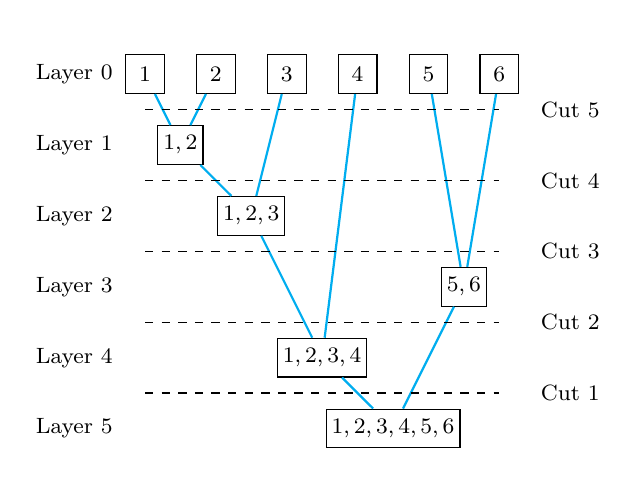
\begin{tikzpicture}[scale=.3, auto,swap]
	% Draw a 7,11 network
	% First we draw the vertices
	\foreach \pos/\name in {{(1*3,0)/1}, {(2*3,0)/2}, {(3*3,0)/3}, {(4*3,0)/4}, {(5*3,0)/5}, {(6*3,0)/6}}
	\node[vertex, rectangle] (\name) at \pos {$\name$};
	\node[vertex, rectangle] (1;2) at (1.5*3,-1*3) {$1, 2$};
	\node[vertex, rectangle] (1;2;3) at (2.5*3,-2*3) {$1, 2, 3$};
	\node[vertex, rectangle] (5;6) at (5.5*3,-3*3) {$5, 6$};
	\node[vertex, rectangle] (1;2;3;4) at (3.5*3,-4*3) {$1, 2, 3, 4$};
	\node[vertex, rectangle] (1;2;3;4;5;6) at (4.5*3,-5*3) {$1, 2, 3, 4, 5, 6$};
	
	% connect vertices with edges and draw weights
	\foreach \source/ \dest  in {
		1/1;2, 2/1;2,
		3/1;2;3, 1;2/1;2;3,
		5/5;6, 6/5;6, 
		1;2;3/1;2;3;4, 4/1;2;3;4,
		1;2;3;4/1;2;3;4;5;6, 5;6/1;2;3;4;5;6}
	\path[edge, thick, cyan] (\source) -- (\dest);
	
	% label
	\node[vertex, note] (layer0) at (0,0) {Layer 0};
	\node[vertex, note] (layer0) at (0,-1*3) {Layer 1};
	\node[vertex, note] (layer0) at (0,-2*3) {Layer 2};
	\node[vertex, note] (layer0) at (0,-3*3) {Layer 3};
	\node[vertex, note] (layer0) at (0,-4*3) {Layer 4};
	\node[vertex, note] (layer0) at (0,-5*3) {Layer 5};
	\node[vertex, note] (cut5) at (7*3,-0.5*3) {Cut 5};
	\node[vertex, note] (cut5) at (7*3,-1.5*3) {Cut 4};
	\node[vertex, note] (cut5) at (7*3,-2.5*3) {Cut 3};
	\node[vertex, note] (cut5) at (7*3,-3.5*3) {Cut 2};
	\node[vertex, note] (cut5) at (7*3,-4.5*3) {Cut 1};
	
	% dash
	\foreach \left / \right in {
		{(1*3,-0.5*3)}/{(6*3,-0.5*3)}, {(1*3,-1.5*3)}/{(6*3,-1.5*3)}, 
		{(1*3,-2.5*3)}/{(6*3,-2.5*3)}, {(1*3,-3.5*3)}/{(6*3,-3.5*3)}, {(1*3,-4.5*3)}/{(6*3,-4.5*3)}}
	\draw [dashed,thin] plot coordinates { \left \right};
	\end{tikzpicture}
	\caption{Example of an agglomerative tree for one class.}
	\label{fig2: tree assignment}
\end{figure}

The problem turns out to find a good similarity estimate between two components which are the groups of word vectors. Denote $S(H, G)$ is the similarity measure function between two groups of word vectors H and G. In other words, the magnitude of $S$ based on the similarity of word distributions on H and G. With each group, we represent it by the means of all vectors in this group. In practice, we use the convenient cosine distance between word vectors. So that 
\begin{align}
s(H, G) = \frac{\sum_{k=1}^{d}{H_i G_i}}{\sqrt{\sum_{k=1}^{d}{H_i^2}} \sqrt{\sum_{k=1}^{d}{G_i^2}}}
\end{align}
Classifier constructs a tree in each label value, then we decide how components are assigned to them.

We continue with the k-means method. In the same logic as hierarchical tree assignment, we construct a k-means clustering on each label value. The method disjoints the data instance of the same label value into the components by minimizing the variance of all data in the same component---minimize the within-cluster sum of squares. For a given label value $y$, denote $\mu^{(j)}$ is the vector mean of all instances in $M_j$ such that $P(y|M_j) = 1$, we have the target of k-means clustering given as
\begin{align}
	\sum_{i=1}^{l}{
		\min_{M_j \in M} {
			\sum_{k=1}^{d}{(x^{(i)}_k - \mu^{(j)}_k)^2}
		}
	}
\end{align}

The next section will provide experimental evidence for our claim on this unsupervised initialization assertion.

\section{Experimental Results}
\label{sec2: exp results}
We set the experiment on three different tasks of 20Newsgroup data set including comp versus rec groups, 8870 instances; comp versus sci groups, 8843 instances and comp versus talk groups, 8144 instances. These are the major label groups in the data set. The text data was constructed with tf-idf vectorizer, the size of vocabulary reduced to 600 words by sum of tf-idf.

In all data cases, we first separate the data into train-test sets with a fixed ratio at 60:40, 60\% of all data for train set and the remaining for test set. After that, the train set continues to split in labeled and unlabeled sets with different split ratio. Both splitting steps also use 5-fold cross validation. We used the splitting ratio of labeled and unlabeled data on train set by the percentage of number of instances in the unlabeled set. For example, the split-70 indicates a split that divides 70\% of instances of train data for unlabeled and 30\% left for labeled. Figure \ref{fig2: data preparing process} gives the overall view of this scheme. In our experiments, we constructed each data case with 3 splits of split-70, split-90 and split-97. In total we have 5-fold for train-test split and 5-fold for each of 3 labeled-unlabeled splitting, $(5 \times 5 \times 3) = 75$ cases for each classifier.
\begin{figure}[ht!]
	\centering
	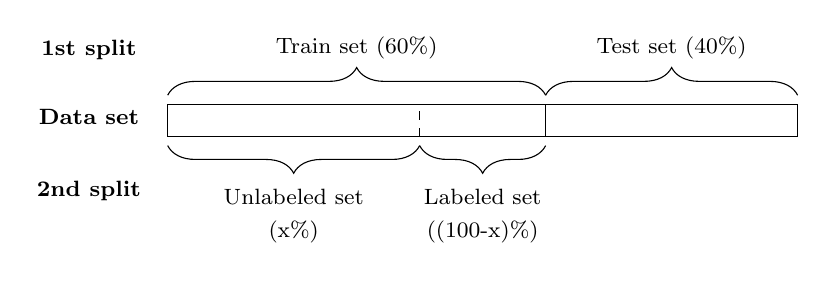
\begin{tikzpicture}[scale=0.8]
		\draw (0,0) rectangle (10,.5) node[midway]{};
		\draw (6,0) -- (6,.5);
		\draw[dashed] (4,0) -- (4,.5);
		
		\draw node[draw=none, xshift=-1cm, yshift=1.1cm] {\footnotesize \textbf{1st split}};
		\draw node[draw=none, xshift=-1cm, yshift=-.7cm] {\footnotesize \textbf{2nd split}};
		\draw node[draw=none, xshift=-1cm, yshift=.25cm] {\textbf{\footnotesize Data set}};
		
		\draw [decorate,decoration={brace,amplitude=10pt}, yshift=0.15cm]
		(0,.5) -- (6,.5) node [black,midway,yshift=0.6cm] {\footnotesize Train set (60\%)};
		\draw [decorate,decoration={brace,amplitude=10pt}, yshift=0.15cm]
		(6,.5) -- (10,.5) node [black,midway,yshift=0.6cm] {\footnotesize Test set (40\%)};
		
		\draw [decorate,decoration={brace,amplitude=10pt, mirror}, , yshift=-0.15cm]
		(0,0) -- (4,0) node [black,midway,yshift=-0.9cm, align=center] {\footnotesize Unlabeled set \\\footnotesize (x\%)};
		\draw [decorate,decoration={brace,amplitude=10pt, mirror}, yshift=-0.15cm]
		(4,0) -- (6,0) node [black,midway,yshift=-0.9cm, align=center] {\footnotesize Labeled set \\\footnotesize ((100-x)\%)};
	\end{tikzpicture}
	\caption{The split-x on a specific data case for multinomial models.}
	\label{fig2: data preparing process}
\end{figure}

The experiments were examined with supervised multinomial Naive Bayes (NB) and the corresponding semi-supervised model with three different initialization methods. They are the conventional randomized (EM-random), hierarchical tree (EM-tree) and k-means clustering (EM-kmeans) assignments. The search component numbers are in $[1, 15]$. Ultimately, we have 3 data cases with 4 inference models, $(3 \times 4) = 12$ classifiers. Since the results are mostly balanced between precision and recall criteria, we only show the measurement of f1-score here. Accordingly, table \ref{table2: exp news 1}, \ref{table2: exp news 2} and \ref{table2: exp news 3} present the results on comp versus rec, comp versus sci and comp versus talk respectively. The complete table of experimental results can be found in appendix \ref{appx: Experiments Resources}.

In all of the data cases and splits, we can observe that the semi-supervised models outperform the supervised NB model. We now consider only the different component initialization methods of semi-supervised classifiers. Starting with the split-70, the performance between the clustering assignments---EM-tree and EM-kmeans---and randomized assignment---EM-random---are merely the same. It is better in some cases, table \ref{table2: exp news 1}, but lower or equal in the others, and the differences are small. The same situation is also in split-90. Finally, with a narrow source of labeled data in split-97, it gives us more clarity to see the advantage of clustering assignment over the random method. Where in most of the cases, we have the better performances in EM-tree and EM-kmeans. In addition, we may notice that in all of the setup, the models show a good adaption with the changes of unlabeled data. On a different scale, the classifiers still keep it performing with small variances.

\pagebreak

\begin{table}[t!]
	\centering
	\captionsetup{justification=centering}
	\caption{Multinomial model evaluation, 20Newsgroups data, \\f1-score measurement, comp versus rec.}
	\makebox[\textwidth][c]{
		\begin{tabular}{ c|cccc }
			Label & \textbf{NB} & \textbf{EM-random} & \textbf{EM-tree} & \textbf{EM-kmeans} \\
			\hline
			
			\multicolumn{1}{c}{} & \multicolumn{4}{c}{Split-70, labeled:unlabeled = 1064:2484} \\
			\hline
			$- 1$ & 0.83 & 0.86 & 0.87 & 0.87 \\
			$+ 1$ & 0.77 & 0.79 & 0.82 & 0.81 \\
			\cline{1-5}
			avg.  & 0.80 & 0.82 & 0.85 & 0.84 \\
			\hline
			
			\multicolumn{1}{c}{} & \multicolumn{4}{c}{Split-90, labeled:unlabeled = 354:3194} \\
			\hline
			$- 1$ & 0.78 & 0.86 & 0.86 & 0.86 \\
			$+ 1$& 0.77 & 0.80 & 0.80 & 0.80 \\
			\cline{1-5}
			avg.  & 0.78 & 0.83 & 0.83 & 0.83 \\
			\hline
			
			\multicolumn{1}{c}{} & \multicolumn{4}{c}{Split-97, labeled:unlabeled = 106:3442} \\
			\hline
			$- 1$ & 0.67 & 0.77 & 0.83 & 0.78 \\
			$+ 1$ & 0.66 & 0.70 & 0.72 & 0.76 \\
			\cline{1-5}
			avg.  & 0.66 & 0.74 & 0.77 & 0.77 \\
			\hline
	\end{tabular}}
	\label{table2: exp news 1}
\end{table}

\begin{table}[t!]
	\centering
	\captionsetup{justification=centering}
	\caption{Multinomial model evaluation, 20Newsgroups data, \\f1-score measurement, comp versus sci.}
	\makebox[\textwidth][c]{
		\begin{tabular}{ c|cccc }
			Label & \textbf{NB} & \textbf{EM-random} & \textbf{EM-tree} & \textbf{EM-kmeans} \\
			\hline
			
			\multicolumn{1}{c}{} & \multicolumn{4}{c}{Split-70, labeled:unlabeled = 1061:2476} \\
			\hline
			$- 1$ & 0.90 & 0.92 & 0.92 & 0.92 \\
			$+ 1$ & 0.85 & 0.89 & 0.89 & 0.89 \\
			\cline{1-5}
			avg. & 0.88 & 0.91 & 0.91 & 0.90 \\
			\hline
			
			\multicolumn{1}{c}{} & \multicolumn{4}{c}{Split-90, labeled:unlabeled = 353:3184} \\
			\hline
			$- 1$ & 0.91 & 0.92 & 0.91 & 0.91 \\
			$+ 1$ & 0.88 & 0.89 & 0.89 & 0.89 \\
			\cline{1-5}
			avg. & 0.89 & 0.90 & 0.90 & 0.90 \\
			\hline
			
			\multicolumn{1}{c}{} & \multicolumn{4}{c}{Split-97, labeled:unlabeled = 106:3431} \\
			\hline
			$- 1$ & 0.88 & 0.89 & 0.91 & 0.91 \\
			$+ 1$ & 0.83 & 0.82 & 0.88 & 0.88 \\
			\cline{1-5}
			avg. & 0.86 & 0.86 & 0.89 & 0.89 \\
			\hline
	\end{tabular}}
	\label{table2: exp news 2}
\end{table}

\begin{table}[t!]
	\centering
	\captionsetup{justification=centering}
	\caption{Multinomial model evaluation, 20Newsgroups data, \\f1-score measurement, comp versus talk.}
	\makebox[\textwidth][c]{
		\begin{tabular}{ c|cccc }
			Label & \textbf{NB} & \textbf{EM-random} & \textbf{EM-tree} & \textbf{EM-kmeans} \\
			\hline
			
			\multicolumn{1}{c}{} & \multicolumn{4}{c}{Split-70, labeled:unlabeled = 977:2280} \\
			\hline
			$- 1$ & 0.94 & 0.95 & 0.94 & 0.95 \\
			$+ 1$ & 0.91 & 0.91 & 0.91 & 0.91 \\
			\cline{1-5}
			avg. & 0.93 & 0.93 & 0.93 & 0.93 \\
			\hline
			
			\multicolumn{1}{c}{} & \multicolumn{4}{c}{Split-90, labeled:unlabeled = 325:2932} \\
			\hline
			$- 1$ & 0.94 & 0.94 & 0.94 & 0.94 \\
			$+ 1$ & 0.89 & 0.91 & 0.90 & 0.91 \\
			\cline{1-5}
			avg. & 0.91 & 0.93 & 0.92 & 0.93 \\
			\hline
			
			\multicolumn{1}{c}{} & \multicolumn{4}{c}{Split-97, labeled:unlabeled = 97:3160} \\
			\hline
			$- 1$ & 0.91 & 0.93 & 0.94 & 0.94 \\
			$+ 1$ & 0.84 & 0.87 & 0.91 & 0.91 \\
			\cline{1-5}
			avg. & 0.88 & 0.90 & 0.92 & 0.92 \\
			\hline
	\end{tabular}}
	\label{table2: exp news 3}
\end{table}
	
	\chapter{Components Separation with Graph}
	We construct a graph $\mathcal{G}$ from the set of instances $\mathcal{X}$, where each data instance is a vertex and the edges represent the relationship between vertices. A model builds on this graph, combines with the information of labeled vertices to estimate the label for unlabeled vertices. In semi-supervised learning, the inferences that utilize the graph structure like this are called graph-based methods.

As an application of graph-based methods, in this chapter, we consider our data assumption in the form of an objective function on $\mathcal{G}$. Then the inference process aims to recognize the boundary between groups of different label vertices.

%The conventional approach solves this function and assigns the label for unlabeled vertices by finding a minimum cut on the graph. Nevertheless, the minimum cut frequently gives an unbalanced assignment when there is more than one solution. The thesis employs the idea of deriving a graphical model on this graph to bypass this problem. Furthermore, the affordable inference on graphical model only works with tree-like graph. Then an approximate algorithm is utilized to deal with the case when our graph does not have the tree form.

%%%%%
\section{Graph Construction}
\label{section3: Graph Construction}

Basically most graph-based methods are transductive learning. A common graph-based setup consists of two basic steps. The first is graph construction where the data is mapped to a graph, $\mathcal{X} \rightarrow \mathcal{G}$. Then in graph inference, we estimate labels for unlabeled data, $\{ \mathcal{G}, \mathcal{Y}_L \} \rightarrow \mathcal{Y}_U$.

In this chapter, we discuss the first step of graph construction. Denote that $n$ is the total number of instances, $n \triangleq l + u$. We initialize a graph $\mathcal{G} = (V, E, W)$, where $V=\{1,  ..., n\}$ is the set of vertices; $E \subseteq V \times V$ is the set of edges and $W$ is a $n \times n$ weight matrix on $E$. First, we need to establish and clarify the basic conditions on $\mathcal{G}$
\begin{description}
	\item[$\mathcal{G}$ is a simple weighted graph:] $\mathcal{G}$ does not contain self-loop and multiple edges; each edge is undirected and assigned with a weight value.
	
	\item[$V$ is constructed from data instances: ] $V$ is constructed by an one-to-one correspondence with data instances and its label, $\{ (\mathcal{X}, \mathcal{Y}) \} \rightarrow V$. This means each vertex contains information of an instance and its corresponding label. In practice, $\mathcal{Y}_U$ is initialized as non-clarified labels $\mathcal{Y}_U = \{ 0 \}^u$.
	
	\item[$W$ is positive and symmetric: ] $W \in \mathbb{R}^{n\times n}, W > 0$ and $W_{i,j} = W_{j,i}$. If $W_{i,j} = 0$ that means there is no edge between $i$ and $j$. In this thesis, we consider the weight on an edge between two vertices as the similarity between them. In other words, the larger the weight is, the more similar the two vertices.
\end{description}

Because the set of vertices $V$ is fixed, the remaining task involves estimating $E$ and $W$. Actually we only take into account the estimation of $W$, because it entirely defines the setup of $E$.

Typically the graph construction process contains two smaller steps: graph sparsification and graph re-weighting. Denote a similarity measure $S: V\times V \rightarrow \mathbb{R}^{n\times n}$ is a function that returns the similarity between two vertices. From the beginning, we initialize $\mathcal{G}$ as a fully connected graph $W_{i,j} = S(x^{(i)}, x^{(j)})$. In graph sparsification, we intend to sparsify $W$ through a binary mass matrix $P \in \{0, 1\}^{n\times n}$, where $P_{i,j} = 1$ means there is an edge between $i$ and $j$ and $0$ otherwise, start with $P$ of all zeros. There are many sparsification algorithms, though we only discuss the primary two that will be set in our practice
\begin{description}
	\item[K-nearest neighbors (kNN):] The typical kNN sparsification searches for the $k$ most similar vertices of each vertex. We set $P_{i,j} = 1$ if $j$ is one of the most similar neighbors of $i$. Also, if $i$ is a selected neighbor of $j$, then the reverse state does not hold. Thus to meet the symmetry condition of $W$, after searching, we have to re-symmetrize $P = max(P, P^T)$. This may lead to the misconception of the result kNN graph when after all we have $\sum_{j}{P_{i,j}} \geq k$, which means the graph would have more edges than expected.
	
	 \item[Maximum spanning tree (MST):] In this construction, we look for a spanning tree---a tree containing all the vertices in $\mathcal{G}$---that has the highest sum of weights. We may further expand this structure by executing the MST on each component of the kNN graph. The benefit of this construction comes from its spanning tree structure, where we always receive the graph with a fixed number of $(n-1)$ edges. But this might be a trade-off if the graph is sparse, it can cause the lost information of vertices connection.
\end{description}

Continuing with the graph re-weighting, from the solution matrix $P$, we continue to re-estimate the weight of the selected edges to produce the final matrix $W$. The motivation of this task is to focus on some target characteristics that we aim at inference step and try to omit the misbehavior of $P$ from sparsification step. There are also some possible approaches to this task \parencite{Jebara:2009:GCB:1553374.1553432, Subramanya:2014:GSL:2765801}. For simplification purposes, we utilize the simplest schedule using the element-wise product to set $W = W \cdot P$. The graph construction process is summarized in algorithm \ref{alg4: graph construction}. It takes the instances set $\mathcal{X}$, label of labeled instances $\mathcal{Y}_L$ and similarity measure $S$ as input and outputs a graph as a pair of vertices set and weight matrix $(V, W)$.
\begin{algorithm}[H]
	\caption{Graph construction process}
	\begin{algorithmic}[1]
		\Function{Graph\_Construction}{$\mathcal{X}, \mathcal{Y}_L, S$}
		
		\State $\mathcal{Y}_U \gets \{0\}^u$
		\COMMENT{Initialize label for unlabeled instances}
		\State $\mathcal{Y} \gets \mathcal{Y}_L \cup \mathcal{Y}_U$
		\COMMENT{Merge the complete label sets}
		\State $V \gets \{(\mathcal{X}, \mathcal{Y})\}$
		\COMMENT{Set $V$ as set of (instance, label)}
		
		\State $W \gets S(V \times V)$
		\COMMENT{Initialize $W$ by similarity measure $S$}
		\State $P = Sparsify(W)$
		\COMMENT{Sparsify $W$}
		\State $W \gets W \cdot P$
		\COMMENT{Re-weigh $W$}
		\RETURN $(V, W)$
		
		\EndFunction
	\end{algorithmic}
	\label{alg4: graph construction}
\end{algorithm}

So far we have been constructing the graph. In the next section we will discuss how to inferring the labels for unlabeled vertices.

%%%%%
\section{Minimum Cut Inference}
\label{section3: mincut approach}

Given our graph after construction $\mathcal{G}$. We presume that the vertices set $V$ is the union of $V_L$ and $V_U$ respectively are the subsets of labeled and unlabeled vertices,  $V = V_L \cup V_U$. Moreover, we assume $U_L = U_{L^+} \cup U_{L^-}$, where $U_{L^+}$ is the positive vertices set and $U_{L^-}$ is the negative vertices set of labeled vertices. We construct a simple target function
\begin{align}
\label{equal4: target function}
\argmin_{f} \quad \frac{1}{2}\sum_{(i,j) \in E}{W_{i,j}|f(i) - f(j)|}
\end{align}
where $f(i) \in \{-1, +1\}$ represents labels for $i \in V$. With $i \in V_L$, $f(i) = -1$ if $i \in U_{L^-}$ and otherwise, $f(i) = +1$ if $i \in U_{L^+}$.

Now let's consider the intuition viewing of  (\ref{equal4: target function}). In \parencite{Blum:2001:LLU:645530.757779}, we have an interesting expression of our implied generative framework in there. We assume that the underlying distribution is a fixed number of combined components---groups of vertices---and each has a unique label. Components are separated by a minimum dissimilarity value. An instance is generated by randomly picking a vertex in one of these components then giving it the label of component which it belongs to. 

The hypothesis here is that with proper graph construction, there is a sparse connection between two components and more densely connected edges inside oneself. Then with a large enough unlabeled data, the component will be more dense and the connection between them will be the loosest one. So they become the boundary to separate the components. Thus, with only a few labeled vertices on each component, we can label all of them. Figure \ref{fig4: combination of components assumption} gives an illustration of this view with four regions of positive and negative labels.
\begin{figure}[!ht]
	\centering
	\begin{subfigure}[b]{0.4\textwidth}
		\centering
		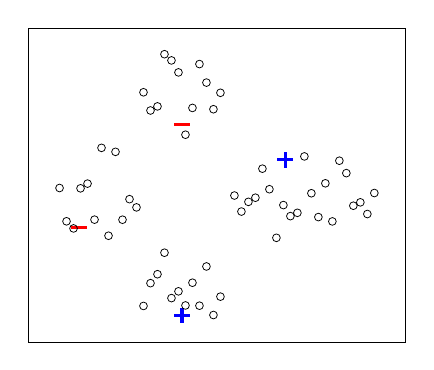
\begin{tikzpicture}[
		scale=.7, auto,swap,
		declare function={a1(\x)=(1 - \x^2)^0.5 - 2;},
		declare function={a2(\x)= -(1 - \x^2)^0.5 - 2;},
		declare function={b1(\x)=(1 - \x^2)^0.5 + 2;},
		declare function={b2(\x)= -(1 - \x^2)^0.5 + 2;},
		declare function={c1(\x)= (1 - (\x + 2)^2)^0.5;},
		declare function={c2(\x)= -(1 - (\x + 2)^2)^0.5;},
		declare function={d1(\x)= (1 - ((\x - 3)^2)/3)^0.5;},
		declare function={d2(\x)= -(1 - ((\x - 3)^2)/3)^0.5;}
		]
		\pgfmathsetseed{1355}
		\begin{axis}[
		% axis line style={draw=none},
		xtick=\empty, ytick=\empty
		]
		\addplot [positive data, samples=5]
		{0.5*(a1(x)+a2(x)) + 0.5*rand*(a1(x)-a2(x))};
		\addplot [positive data, samples=5]
		{0.5*(d1(x)+d2(x)) + 0.5*rand*(d1(x)-d2(x))};
		\addplot [unlabeled data, samples=60]
		{0.5*(a1(x)+a2(x)) + 0.5*rand*(a1(x)-a2(x))};
		\addplot [unlabeled data, samples=60]
		{0.5*(d1(x)+d2(x)) + 0.5*rand*(d1(x)-d2(x))};
		
		\addplot [negative data, samples=5]
		{0.5*(b1(x)+b2(x)) + 0.5*rand*(b1(x)-b2(x))};
		\addplot [negative data, samples=5]
		{0.5*(c1(x)+c2(x)) + 0.5*rand*(c1(x)-c2(x))};
		\addplot [unlabeled data, samples=60]
		{0.5*(b1(x)+b2(x)) + 0.5*rand*(b1(x)-b2(x))};
		\addplot [unlabeled data, samples=60]
		{0.5*(c1(x)+c2(x)) + 0.5*rand*(c1(x)-c2(x))};
		\end{axis}
		\end{tikzpicture}
		\caption{}
		\label{fig4.a: combination of components assumption}
	\end{subfigure}
	\begin{subfigure}[b]{0.4\textwidth}
		\centering
		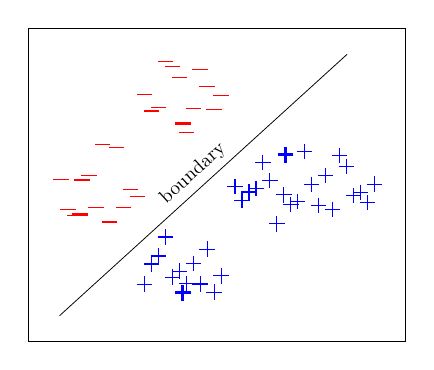
\begin{tikzpicture}[
		scale=.7, auto,swap,
		declare function={a1(\x)=(1 - \x^2)^0.5 - 2;},
		declare function={a2(\x)= -(1 - \x^2)^0.5 - 2;},
		declare function={b1(\x)=(1 - \x^2)^0.5 + 2;},
		declare function={b2(\x)= -(1 - \x^2)^0.5 + 2;},
		declare function={c1(\x)= (1 - (\x + 2)^2)^0.5;},
		declare function={c2(\x)= -(1 - (\x + 2)^2)^0.5;},
		declare function={d1(\x)= (1 - ((\x - 3)^2)/3)^0.5;},
		declare function={d2(\x)= -(1 - ((\x - 3)^2)/3)^0.5;}
		]
		\pgfmathsetseed{1355}
		\begin{axis}[
%		 axis line style={draw=none},
		xtick=\empty, ytick=\empty
		]
		\addplot [positive data, samples=5]
		{0.5*(a1(x)+a2(x)) + 0.5*rand*(a1(x)-a2(x))};
		\addplot [positive data, samples=5]
		{0.5*(d1(x)+d2(x)) + 0.5*rand*(d1(x)-d2(x))};
		\addplot [positive data, samples=60, style=semithick]
		{0.5*(a1(x)+a2(x)) + 0.5*rand*(a1(x)-a2(x))};
		\addplot [positive data, samples=60, style=semithick]
		{0.5*(d1(x)+d2(x)) + 0.5*rand*(d1(x)-d2(x))};
		
		\addplot [negative data, samples=5]
		{0.5*(b1(x)+b2(x)) + 0.5*rand*(b1(x)-b2(x))};
		\addplot [negative data, samples=5]
		{0.5*(c1(x)+c2(x)) + 0.5*rand*(c1(x)-c2(x))};
		\addplot [negative data, samples=60, style=semithick]
		{0.5*(b1(x)+b2(x)) + 0.5*rand*(b1(x)-b2(x))};
		\addplot [negative data, samples=60, style=semithick]
		{0.5*(c1(x)+c2(x)) + 0.5*rand*(c1(x)-c2(x))};
		
		% bound
    	\addplot[mark=none] coordinates { (-3,-3) (4,3) } node [midway, sloped, above] {boundary};

		\end{axis}
		\end{tikzpicture}
		\caption{}
		\label{fig4.b: combination of components assumption}
	\end{subfigure}
	\hfill
	\caption[Illustration of the combination of graph components assumption.]{Illustration of the combination of graph components assumption. There are two positive and two negative regions. When there is enough unlabeled data, each component will form as a dense graph---figure (a). Then with only one labeled vertex on each component, we can decide the boundary and label all unlabeled vertices---figure (b).}
	\label{fig4: combination of components assumption}
\end{figure}

We are now looking for the inference which can be adapted to the optimization condition (\ref{equal4: target function}) above. Literally, the solution is a configuration of $f(i), i \in V_U$ that guarantees the minimization. With a small set of unlabeled data, a brute-force approach that finds all the $2^u$ configurations of unlabeled vertices seems like a possible solution. But the basic condition of semi-supervised learning is a large scale of $u$. A common solution for this inference is the mincut approach using a minimum cut on $\mathcal{G}$ \parencite{Blum:2001:LLU:645530.757779}. It finds a minimum cut on which it separates all positive and negative vertices. Recall a cut $C= \{C_1, C_2\}$ on $\mathcal{G}$ is a segmentation of $V$ such that $C_1 \cap C_2 = \emptyset, C_1 \cup C_2 = V$. The size of cut $C$ is the total weight of edges between $C_1$ and $C_2$. More precisely, denote $W_C$ is the size of the cut, we have $W_C = \sum_{i \in C_1, j \in C_2} W_{i,j}$. Given a pair of source and sink vertices $(s, t)$, the minimum cut algorithm finds a cut with smallest weight such that $s \in C_1$ and $t \in C_2$. The solution for finding minimum cut is a well-known algorithm in graph theory and can be archived in polynomial running time. The detailed descriptions and tutorials of this algorithm can be found in \parencite{cormen2009introduction, West2001}.

Define that $MinCut(\mathcal{G}, s, t)$ is a function which searches for a minimum cut on $\mathcal{G}$ with source vertex $t$ and sink vertex $s$. The output returns a cut $C$ with $s \in C_1$ and $t \in C_2$. The mincut approach starts by adding two new pseudo vertices $v_+$ and $v_-$ to $V$, then connects $v_+$ with all positive and $v_-$ with all negative vertices. These pseudo vertices are treated as pins that keep all positive and negative vertices in separate parts. When we have a minimum cut on $\mathcal{G}$ with $v_+$ and $v_-$ are source and sink, MinCut$(\mathcal{G}, v_+, v_-)$. We can label all unlabeled vertices using its correspondence with $v_+$ or $v_-$. All vertices in the part containing $v_+$ will have the positive label and all vertices in the part of $v_-$ will have the negative label. Figure \ref{fig4: mincut example} illustrates the process of mincut approach and we summarize the process in algorithm \ref{alg4: mincut}. It receives the graph $\mathcal{G}$ as input and returns the vertices set $V$ after labeling all unlabeled vertices.

It is obvious that the complexity of this approach mainly comes from the function MinCut$(\mathcal{G}, s, t)$. Constantly, the problem of finding a minimum s-t cut in graph is similar to looking for a maximum flow on $\mathcal{G}$. For a quick implementation, we may take the well known Edmonds–Karp algorithm \parencite{Edmonds:1972:TIA:321694.321699} which costs us $\mathcal{O}(n|E|^2)$ to find the solution. One of the more advanced methods, the push-relabel algorithm \parencite{KING1994447}, is commonly supported in difference graph frameworks having the complexity of $\mathcal{O}(n|E|\log{\frac{n^2}{|E|}})$. There are also other methods that would save more time, but they are far more complicated to be considered in our meaning time.

\begin{figure}[!ht]
	\centering
	\captionsetup[subfigure]{justification=centering}
	\begin{subfigure}[b]{0.4\textwidth}
		\centering
		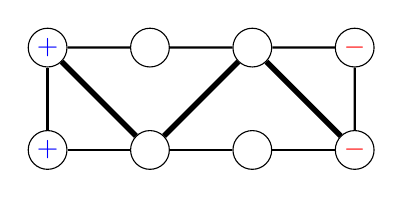
\begin{tikzpicture}[scale=1.3, auto,swap]
		% First we draw the vertices
		\foreach \pos/\label/\name in {
			{(0,0)/a/+}, {(1,0)/b/}, {(2,0)/c/},
			{(0,1)/e/+}, {(1,1)/f/}, {(2,1)/g/}}
		\node[positive vertex] (\label) at \pos{$\name$};
		
		\foreach \pos/\label/\name in {{(3,0)/d/-}, {(3,1)/h/-}}
		\node[negative vertex] (\label) at \pos{$\name$};
		
		% Connect vertices with edges and draw weights
		\foreach \source/ \dest in {
			b/e,b/g,d/g}
		\path[thickedge] (\source) -- (\dest);
		\foreach \source/ \dest in {
			a/b,a/e,b/c,c/d,d/h,e/f,f/g,g/h}
		\path[edge] (\source) -- (\dest);
		\end{tikzpicture}
		\caption*{Input graph $G$, weight is represented as edge thickness.}
	\end{subfigure}
	\hfill
	\begin{subfigure}[b]{0.5\textwidth}
		\centering
		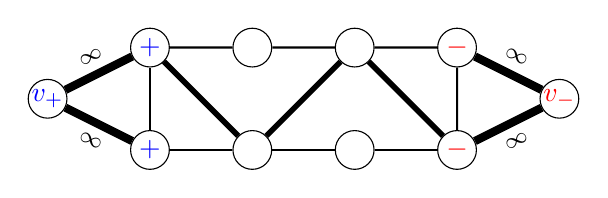
\begin{tikzpicture}[scale=1.3, auto,swap]
		% First we draw the vertices
		\foreach \pos/\label/\name in {
			{(0,0)/a/+}, {(1,0)/b/}, {(2,0)/c/},
			{(0,1)/e/+}, {(1,1)/f/}, {(2,1)/g/}, {(-1,0.5)/v+/v_+}}
		\node[positive vertex] (\label) at \pos{$\name$};
		
		\foreach \pos/\label/\name in {{(3,0)/d/-}, {(3,1)/h/-}, {(4,0.5)/v-/v_-}}
		\node[negative vertex] (\label) at \pos{$\name$};
		
		% Connect vertices with edges and draw weights
		\foreach \source/ \dest in {
			b/e,b/g,d/g}
		\path[thickedge] (\source) -- (\dest);
		\foreach \source/ \dest in {
			a/b,a/e,b/c,c/d,d/h,e/f,f/g,g/h}
		\path[edge] (\source) -- (\dest);
		
		% inf weight
		\path[draw, line width=3pt] (v+) -- node[sloped, above]{\footnotesize $\infty$} (e);
		\path[draw, line width=3pt] (v-) -- node[sloped, above]{\footnotesize $\infty$} (h);
		
		\path[draw, line width=3pt] (v+) -- node[sloped, below]{\footnotesize $\infty$} (a);
		\path[draw, line width=3pt] (v-) -- node[sloped, below]{\footnotesize $\infty$} (d);
		\end{tikzpicture}
		\caption*{Step 1, add pseudo vertices $v_+, v_-$ and corresponding edges.}
	\end{subfigure}

	\vspace*{5pt}
	\begin{subfigure}[b]{0.5\textwidth}
		\centering
		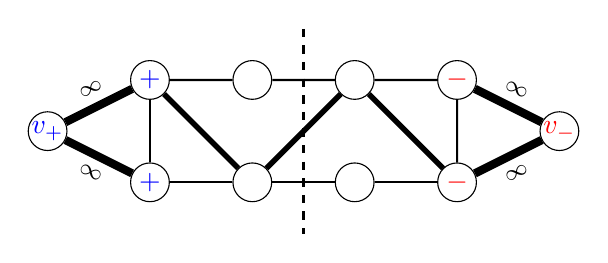
\begin{tikzpicture}[scale=1.3, auto,swap]
		% First we draw the vertices
		\foreach \pos/\label/\name in {
			{(0,0)/a/+}, {(1,0)/b/}, {(2,0)/c/},
			{(0,1)/e/+}, {(1,1)/f/}, {(2,1)/g/}, {(-1,0.5)/v+/v_+}}
		\node[positive vertex] (\label) at \pos{$\name$};
		
		\foreach \pos/\label/\name in {{(3,0)/d/-}, {(3,1)/h/-}, {(4,0.5)/v-/v_-}}
		\node[negative vertex] (\label) at \pos{$\name$};
		
		% Connect vertices with edges and draw weights
		\foreach \source/ \dest in {
			b/e,b/g,d/g}
		\path[thickedge] (\source) -- (\dest);
		\foreach \source/ \dest in {
			a/b,a/e,b/c,c/d,d/h,e/f,f/g,g/h}
		\path[edge] (\source) -- (\dest);
		
		% inf weight
		\path[draw, line width=3pt] (v+) -- node[sloped, above]{\footnotesize $\infty$} (e);
		\path[draw, line width=3pt] (v-) -- node[sloped, above]{\footnotesize $\infty$} (h);
		
		\path[draw, line width=3pt] (v+) -- node[sloped, below]{\footnotesize $\infty$} (a);
		\path[draw, line width=3pt] (v-) -- node[sloped, below]{\footnotesize $\infty$} (d);
		
		\path[dashedge] (1.5, 1.5) -- (1.5, -0.5);
		\end{tikzpicture}
		\caption*{Step 2, find a minimum cut in G with source $v_+$ and sink $v_-$.}
	\end{subfigure}
	\hfill
	\begin{subfigure}[b]{0.4\textwidth}
		\centering
		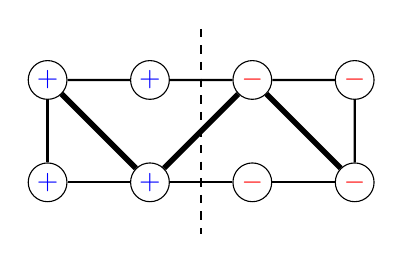
\begin{tikzpicture}[scale=1.3, auto,swap]
		% First we draw the vertices
		% First we draw the vertices
		\foreach \pos/\label/\name in {
			{(0,0)/a/+}, {(0,1)/e/+}, {(1,0)/b/+}, {(1,1)/f/+}}
		\node[positive vertex] (\label) at \pos{$\name$};
		
		\foreach \pos/\label/\name in {
			{(3,0)/d/-}, {(3,1)/h/-}, {(2,1)/g/-}, {(2,0)/c/-}}
		\node[negative vertex] (\label) at \pos{$\name$};
		
		% Connect vertices with edges and draw weights
		\foreach \source/ \dest in {
			b/e,b/g,d/g}
		\path[thickedge] (\source) -- (\dest);
		\foreach \source/ \dest in {
			a/b,a/e,b/c,c/d,d/h,e/f,f/g,g/h}
		\path[edge] (\source) -- (\dest);
		
		\path[dashedge] (1.5, 1.5) -- (1.5, -0.5);
		\end{tikzpicture}
		\caption*{Step 3, use this cut to label unlabeled vertices.}
	\end{subfigure}
	\caption{Example of mincut approach.}
	\label{fig4: mincut example}
\end{figure}

\begin{algorithm}[H]
	\caption{Semi-supervised mincut approach}
	\begin{algorithmic}[1]
		\Function{Mincut\_SSL}{$\mathcal{G}, s, t$}
		\State \texttt{\# Step 1}
		\State{$V \gets V \cup \{v_+, v_-\}$}
		\COMMENT{Add in $\mathcal{G}$ two new vertices $v_+$ and $v_-$}
		\For{$i \in V_{L^+}$}
		\COMMENT{For each positive vertices:}
		\State{$W_{i, v_+} \gets +\infty$}
		\COMMENT{Connect to $v_+$ with $+\infty$ weight}
		\EndFor
		\For{$i \in V_{L^-}$}
		\COMMENT{For each negative vertices:}
		\State{$W_{i, v_-} \gets +\infty$}
		\COMMENT{Connect to $v_-$ with $+\infty$ weight}
		\EndFor
		
		\State \texttt{\# Step 2}
		\State{$C = MinCut(\mathcal{G}, v_+, v_-)$}
		\COMMENT{Find a minimum cut on $\mathcal{G}$ }
		
		\State \texttt{\# Step 3}
		\For{$i \in C_1$}
		\COMMENT{For each vertex in the part contains $v_+$:}
		\State{$V_{L^+} \gets V_{L^+} \cup i$}
		\COMMENT{Add to the positive label set}
		\EndFor
		\For{$i \in C_2$}
		\COMMENT{For each vertex in the part contains $v_-$:}
		\State{$V_{L^-} \gets V_{L^-} \cup i$}
		\COMMENT{Add to the negative label set}
		\EndFor
		\State{$V \gets V_{L^+} \cup V_{L^-}$}
		\COMMENT{$V$ is now all labeled}
		\RETURN $V$
		
		\EndFunction
	\end{algorithmic}
	\label{alg4: mincut}
\end{algorithm}

In the case of having more than one minimum cut, which means more than one configuration of $f$ that matches the condition (\ref{equal4: target function}), the mincut approach is prone to a cut that is close to the positive or negative region. Thus this label will have a smaller proportion of vertices. For instance, in figure \ref{fig4: mincut unbalance}, the selected cut is more likely to be $C_1$ or $C_2$ than others. From an overall perspective, this missing behavior may not tell much about the performance of this approach, since we do not know the exact global proportion of data set. However, many experiments had been conducted on this problem and showed that it is better to have the solution with more balance between labels \parencite{Blum:2001:LLU:645530.757779, Blum:2004:SLU:1015330.1015429, Joachims:2003:TLV:3041838.3041875, Malik2000}. Furthermore, the balanced cut solution has been proved to be an NP-hard problem \parencite{Malik2000}.

\begin{figure}[ht!]
	\centering
	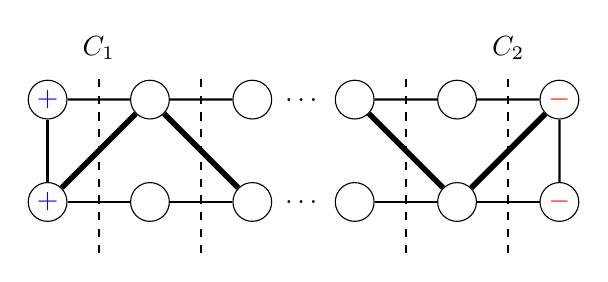
\begin{tikzpicture}[scale=1.3, auto,swap]
	% First we draw the vertices
	\foreach \pos/\label/\name in {
		{(0,0)/a/+}, {(1,0)/b/}, {(2,0)/c/}, {(3,0)/d/}, {(4,0)/e/},
		{(0,1)/g/+}, {(1,1)/h/}, {(2,1)/i/}, {(3,1)/j/}, {(4,1)/k/}}
	\node[positive vertex] (\label) at \pos{$\name$};
	
	\foreach \pos/\label/\name in {{(5,0)/f/-}, {(5,1)/l/-}}
	\node[negative vertex] (\label) at \pos{$\name$};
	
	\foreach \pos/\label in {{(2.5, 0)/x1}, {(2.5, 1)/x2}}
	\node (\label) at \pos{$\dots$};
		
	% Connect vertices with edges and draw weights
	\foreach \source/ \dest in {
		a/h, h/c, j/e, e/l}
	\path[thickedge] (\source) -- (\dest);
	\foreach \source/ \dest in {
		a/b, b/c, d/e, e/f, f/l, l/k, k/j, i/h, h/g, g/a}
	\path[edge] (\source) -- (\dest);
	
	\path[dashedge] (.5, 1.2) -- (.5, -0.5);
	\node[note] at (.5,1.5) {$C_1$};
	\path[dashedge] (1.5, 1.2) -- (1.5, -0.5);
	\path[dashedge] (3.5, 1.2) -- (3.5, -0.5);
	\path[dashedge] (4.5, 1.2) -- (4.5, -0.5);
	\node[note] at (4.5,1.5) {$C_2$};
	\end{tikzpicture}
	\caption{Example of a graph has more than one minimum cut.}
	\label{fig4: mincut unbalance}
\end{figure}

In \parencite{Blum:2004:SLU:1015330.1015429}, we have an idea of the \textit{randomized mincut approach}. The method repeatedly disturbs the edges set $E$ by adding a small amount of noise into the weight matrix. At each iteration, it finds a new minimum cut. The cut is then verified and will be removed if it gives an unbalanced prediction on the train set. Finally, with a set of cuts, the label will be decided on the majority agreements of all cuts. However, through our experimental investigation, this method has no advantage over the original mincut approach. Following this unbalanced issue, in the next chapter, we are going to examine an alternative solution for the mincut approach.

%%%%%
\section{Graphical Model}

A possible replacement for the mincut approach employs a graphical model. This idea was raised by \citeauthor{Blum:2001:LLU:645530.757779} \parencite{Blum:2001:LLU:645530.757779} and had the first fundamental experimental verification with a tree graph construction in \parencite{Blum:2004:SLU:1015330.1015429}. Graphical model is a wide range of research field which is approaching the graph structure on exploring the connected relationship of a set of random variables. This thesis does not try to cover the general technical terms and algorithms of this model. Accordingly, it only focuses on the application of this model in case of solving the target function on binary classification. Gentle introductions, tutorials and examples for graphical model can be found in \parencite{jordan2004, Koller2009, bishop2006pattern}.

Currently, the conventional deployment of graphical model on (\ref{equal4: target function}) only works with a graph forming as a tree using \textit{max-sum} algorithm. The algorithm itself does not have much ability to adapt to the balancing problem. This thesis introduces the \textit{influence index} that supports the inference decision on each vertex when we have more than one applicable decision. In addition, there is no affordable learning algorithm that can work on an arbitrary graph. To complement the conventional approach, we extend this approach in the case of graph having cycles using the approximate inference algorithm \textit{loopy belief propagation}. Combine them together and we have a complete alternative solution for the mincut approach that can be assembled with general graph constructions. Algorithm \ref{alg4: graphical model combination} gives a brief sketch for this combination.
\begin{algorithm}[H]
	\caption{Graphical model for arbitrary graph using influence index}
	\begin{algorithmic}[1]
		\Function{GraphicalModel\_SSL}{$\mathcal{G}, y_L$}
		\State{influence $\gets$ \textless Extract influence index for $i \in V_U$\textgreater}
		\If{$\mathcal{G}$  \textbf{is} Tree}
		\State{$ \textnormal{inference} \gets \textnormal{Max\_Sum}(\mathcal{G}, y_L, \textnormal{influence})$}
		\Else
		\State{$ \textnormal{inference} \gets \textnormal{Loopy\_Belief}(\mathcal{G}, y_L)$}
		\EndIf
		\State{$y_U \gets$ \textless Trace back label from inference\textgreater}
		\RETURN $y_U$
		
		\EndFunction
	\end{algorithmic}
	\label{alg4: graphical model combination}
\end{algorithm}

\subsection{Inference on Tree}
To keep this chapter consistent and self-contained, we first go through with the model setup and the fundamental idea of the max-sum algorithm. Suppose we have a set of random variables $X = \{X_i : i \in V, X_i = f(i) \}$. Define a set of factors
\begin{align}
	\Phi = \{ \phi_{i,j} : (i,j) \in E, \phi_{i,j} = \exp(-W_{i,j}(X_i - X_j)^2) \}
\end{align}
We assume that the implied distribution of $X_i$ only depends on $\Phi$; $\phi(u,v)$ is independent at each other. We can define our model as a joint distribution
\begin{align}
	\label{equal4: graphical model}
	& P_\Phi(X) = \frac{1}{Z} \prod_{(i,j) \in E}{\phi_{i,j}} \\
	\intertext{where the normailizing constant (partition function)}
	&Z = \sum_{X} \prod_{(i,j) \in E}{\phi_{i,j}}\nonumber
\end{align}

Consider the inference to maximize the joint distribution
\begin{align}
	\begin{split}
	\argmax_X{P_\Phi}(X) & = \argmax_X{\frac{1}{Z} \prod_{(i,j) \in E}{\phi_{i,j}}} \\
	& =  \argmax_X{\prod_{(i,j) \in E}{\phi_{i,j}}}
	\end{split}
	\label{equal4: MAP graphical model}
\end{align}
Take the logarithm, then we have
\begin{align}
	\begin{split}
	(\ref{equal4: MAP graphical model}) &= \argmax_X{\ln(\prod_{(i,j) \in E}{\phi_{i,j}})} \\
	&= \argmax_X{\ln(\prod_{(i,j) \in E}{ \exp(-W_{i,j}(X_i - X_j)^2) })} \\
	&= \argmax_X{\sum_{(u,v) \in E}{ -W_{i,j}(X_i - X_j)^2 }}
	\end{split}
	\label{equal4: log MAP}
\end{align}
Combine the condition $W_{u,v}(X_u - X_v)^2 \geq 0$, then from (\ref{equal4: log MAP}) we can obtain that the result of this inference is similar to our target function (\ref{equal4: target function}).

Looking back at our inference (\ref{equal4: MAP graphical model}), define $X_{max}$ is an observed set of $X$ that maximizes the joint distribution, we have
\begin{align}
	X_{max} = \argmax_X{P_\Phi}(X)
\end{align}
Then from (\ref{equal4: graphical model}), the maximize probability can be represented as
\begin{align}
	\begin{split}
	P_\Phi(X_{max}) &= \max_X{P_\Phi}\\
	&= \max_{X_1, ..., X_n}{\prod_{(i,j) \in E}{\phi_{i,j}}}
	\end{split}
	\label{equal4: expanded maximize join distribution}
\end{align}

Let's consider a simple case when we have a tree as a chain of vertices in figure \ref{fig4.a: chain graph}, we have
\begin{align}
		(\ref{equal4: expanded maximize join distribution}) &\Leftrightarrow 
		\max_{X_1, ..., X_n}{\left( \phi_{1,2} \ \phi_{2,3} \dots \phi_{m-1,m} \ \phi_{m,m+1} \dots \phi_{n-1,n} \right)}\\
		& = \max_{X_1} \left[ \max_{X_2} \left[ \dots \left[ 
			\max_{X_n}{ \left( \phi_{1,2} \ \phi_{2,3} \dots \phi_{m-1,m} \ \phi_{m,m+1} \dots \phi_{n-1,n} \right) }
		\right] \dots \right] \right]
		\label{equal4: chain tree: inference equation}
\end{align}

\begin{figure}[!ht]
	\centering
	\begin{subfigure}[b]{\textwidth}
		\centering
		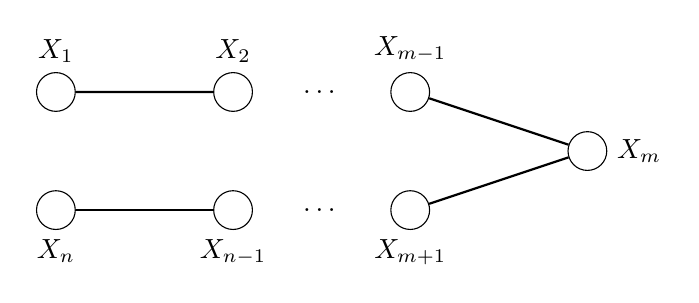
\begin{tikzpicture}[scale=1.5, auto,swap]
		% First we draw the vertices
		\foreach \pos/\label/\name in {
			{(0,1)/a/X_1}, {(1.5,1)/b/X_2}, {(3,1)/c/X_{m-1}}}
		\node[vertex, label={$\name$}] (\label) at \pos{};
		
		\node[vertex, label=right:{$X_m$}] (d) at (4.5,0.5){};
		
		\foreach \pos/\label/\name in {
			{(0,0)/g/X_n}, {(1.5,0)/f/X_{n-1}}, {(3,0)/e/X_{m+1}}}
		\node[vertex, label=below:{$\name$}] (\label) at \pos{};
		
		\foreach \pos in {(2.25, 0), (2.25, 1)}
		\node at \pos{$\dots$};
		
		% Connect vertices with edges 
		\foreach \source/ \dest in {
			a/b, c/d, g/f, e/d}
		\path[edge] (\source) -- (\dest);
		\end{tikzpicture}
		\caption{A simple graph forms a chain of vertices.}
		\label{fig4.a: chain graph}
	\end{subfigure}

	\hfill

	\begin{subfigure}[b]{\textwidth}
		\centering
		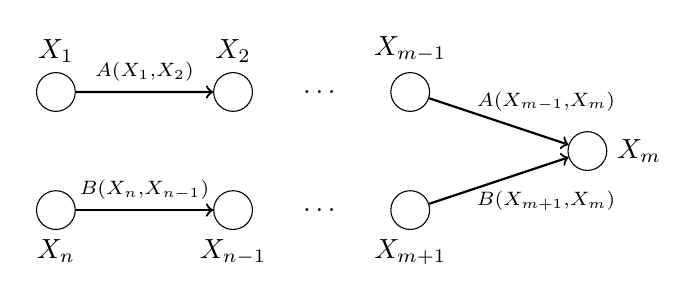
\begin{tikzpicture}[scale=1.5, auto,swap]
		% First we draw the vertices
		\foreach \pos/\label/\name in {
			{(0,1)/a/X_1}, {(1.5,1)/b/X_2}, {(3,1)/c/X_{m-1}}}
		\node[vertex, label={$\name$}] (\label) at \pos{};
		
		\node[vertex, label=right:{$X_m$}] (d) at (4.5,0.5){};
		
		\foreach \pos/\label/\name in {
			{(0,0)/g/X_n}, {(1.5,0)/f/X_{n-1}}, {(3,0)/e/X_{m+1}}}
		\node[vertex, label=below:{$\name$}] (\label) at \pos{};
		
		\foreach \pos in {(2.25, 0), (2.25, 1)}
		\node at \pos{$\dots$};
		
		% Connect vertices with edges 
		\foreach \source/ \dest/ \name  in {
			a/b/{A(X_1,X_2)}, g/f/{B(X_{n},X_{n-1})}}
		\path[edge, ->] (\source) -- (\dest) node[midway, above]{$\scriptstyle \name$};
		
		% Connect vertices with edges
		\path[edge, ->] (e) -- (d) node[midway, below, xshift=6mm]{$\scriptstyle B(X_{m+1},X_m)$};
		\path[edge, ->] (c) -- (d) node[midway, above, xshift=6mm]{$\scriptstyle A(X_{m-1},X_m)$};
		\end{tikzpicture}
		\caption{Messages send from $X_1$ to $X_m$ and from $X_n$ to $X_m$}
		\label{fig4.b: message sending as A and B}
	\end{subfigure}
	\caption{Inference in a chain of vertices.}
	\label{fig4: tree as chain of vertices}
\end{figure}

We first assume that all the random variables are unobserved. Follow the maximization of all random variables in (\ref{equal4: chain tree: inference equation}) gives a brute force approach that takes all positive combination of $X$ having $2^n$ cases. Now we are looking for a better way to compute it. We may have noticed that each maximization on a random variable only affects on the factor functions which have this variable as one of its parameters and there are at most two factors that is related to a maximization. For example, the maximization on $X_m$ only affects on $\phi_{m-1, m}$ and $\phi_{m, m+1}$. Furthermore, in figure \ref{fig4.a: chain graph}, we have two special random variables that belong to only one factor, $X_1$ and $X_n$. Also, they are corresponding with two leaf vertices on this tree. Then we can rearrange (\ref{equal4: chain tree: inference equation}) to group only related factors with its maximization, so that
\begin{align}
	\begin{split}
		(\ref{equal4: chain tree: inference equation}) = \max_{X_m} \biggl[
		& \max_{X_{m-1}}{
			\phi_{m-1, m} \left[ \dots \left[  \max_{X_2}{
				\phi_{2,3} \left( \max_{X_1}{\phi_{1,2}} \right)
			} \right] \dots \right]
		} \\
		& \max_{X_{m+1}}{
			\phi_{m+1, m} \left[ \dots \left[  \max_{X_{n-1}}{
				\phi_{n-1,n-2} \left( \max_{X_n}{\phi_{n,n-1}} \right)
			} \right] \dots \right]
		}
		\biggr]
	\end{split}
	\label{equal4: chain tree: rearrange inference}
\end{align}
We may observe that (\ref{equal4: chain tree: rearrange inference}) contains two parts, the first part is group of maximization of $[X_1, ..., X_{m-1}]$ and the second part is of $[X_{m+1}, ..., X_{n}]$. Consider the first part, we define a function $A$ recursively
\begin{align*}
	& A(X_1, X_2) = \max_{X_1}{\phi_{1,2}}, \\
	& A(X_2, X_3) = \max_{X_2}{\left( \phi_{2,3}A(X_1, X_2) \right)}, \\
	& ..., \\
	& A(X_{m-1}, X_m) = \max_{X_{m-1}}{\left( \phi_{m-1,m}A(X_{m-2}, X_{m-1}) \right)}
\end{align*}
Similarly, we define a function $B$ for the second group
\begin{align*}
	& B(X_n, X_{n-1}) = \max_{X_n}{\phi_{n,n-1}}, \\
	& B(X_{n-1}, X_{n-2}) = \max_{X_{n-1}}{\left( \phi_{n-1,n-2}B(X_{n}, X_{n-1}) \right)}, \\
	& ..., \\
	& B(X_{m+1}, X_m) = \max_{X_{m+1}}{\left( \phi_{m+1,m}B(X_{m+2}, X_{m+1}) \right)}
\end{align*}
Combine them together and we have
\begin{align}
	(\ref{equal4: chain tree: rearrange inference}) \Leftrightarrow \max_{X_m}{\left( 
		A(X_{m-1}, X_m) B(X_{m+1}, X_m) 
		\right)}
\end{align}
Consequently, the inference through recursive functions $A$ and $B$ reduces our calculation significantly. The size of each maximization now is $2^2 = 4$ cases---a factor that inputs 2 variables and each has value in $\{-1, 1\}$---and we only need to execute it $|E|$ times. In addition, we may consider $A$ and $B$ as messages sent on the graph, $A$ is messages sent from vertex of $X_1$ to $X_m$ and $B$ is messages sent from vertex of $X_n$ to $X_m$. The figure \ref{fig4.b: message sending as A and B} shows this view of message sending process. 

Let's formalize this idea to a general tree. At first, on each edge, we need to decide a sending schedule where message will be sent starting from the leaf vertices to a root. Moreover, the sending schedule follows the condition that before a message is sent from a vertex, it must receive all the messages sent to it. We can handle this schedule using a breadth-first search starting from any vertex as the root and invert the search route to get the sending schedule. Figure \ref{fig4: types of vertices on tree} summarizes the different types of vertices we need to handle in this sending process.

\begin{figure}[ht!]
	\centering
	\begin{subfigure}[b]{.3\textwidth}
		\centering
		\begin{tikzpicture}[scale=1.5, auto,swap]
		% First we draw the vertices
		\node[vertex, label={$X_i$}] (a) at (0,0){};
		\node (b) at (1, 0){$\dots$};
		\path[edge, ->] (a) -- (b);
		\node[ellipse, minimum height=3cm, minimum width=1cm] at (0,0) {};
		\end{tikzpicture}
		\caption{A leaf vertex}
		\label{fig4.a: types of vertices on tree: leaf}
	\end{subfigure}
	\hfill
	\begin{subfigure}[b]{.3\textwidth}
		\centering
		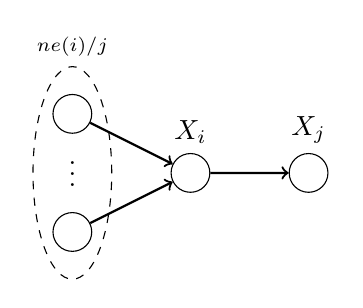
\begin{tikzpicture}[scale=1.5, auto,swap]
		% First we draw the vertices
		\foreach \pos/\label in {
			{(0,0)/a}, {(0,1)/b}}
		\node[vertex] (\label) at \pos{};
		\node at (0,0.56){$\vdots$};
		
		\node[dashed, draw, ellipse, 
		minimum height=2.7cm, minimum width=1cm,
		label=above:{$\scriptstyle ne(i)/j$}] at (0,0.5) {};
		
		\foreach \pos/\label/\name in {
			{(1,0.5)/i/X_i}, {(2,0.5)/j/X_j}}
		\node[vertex, label={$\name$}] (\label) at \pos{};
				
		\foreach \source/ \dest in {
			a/i, b/i, i/j}
		\path[edge, ->] (\source) -- (\dest);
		\end{tikzpicture}
		\caption{A typical vertex}
		\label{fig4.b: types of vertices on tree: normal vertex}
	\end{subfigure}
	\hfill
	\begin{subfigure}[b]{.3\textwidth}
		\centering
		\begin{tikzpicture}[scale=1.5, auto,swap]
		% First we draw the vertices
		\foreach \pos/\label in {
			{(0,0)/a}, {(0,1)/b}}
		\node[vertex] (\label) at \pos{};
		\node at (0,0.56){$\vdots$};
		
		\node[dashed, draw, ellipse, 
		minimum height=2.7cm, minimum width=1cm,
		label=above:{$\scriptstyle ne(m)$}] at (0,0.5) {};
		
		\foreach \pos/\label/\name in {
			{(1,0.5)/m/X_m}}
		\node[vertex, label={$\name$}] (\label) at \pos{};
		
		\foreach \source/ \dest in {
			a/i, b/i}
		\path[edge, ->] (\source) -- (\dest);
		\end{tikzpicture}
		\caption{The root vertex}
		\label{fig4.c: types of vertices on tree: root}
	\end{subfigure}
	
	\caption{Types of vertices on a tree.}
	\label{fig4: types of vertices on tree}
\end{figure}

Assume that a message is sent from $i$ to $j$. Then on edge $(i,j) \in E$  which is not a leave or root vertex, we define the message
\begin{align}
\psi(X_i, X_j) = \max_{X_i} \left[ 
\phi_{i,j} \prod_{k \in ne(i)/j} {\psi(X_k, X_i)}
\right]
\label{equal4: product message on vertex}
\end{align}
Where $ne(i)$ is a function returns set of all neighbor vertices of $i$. In practice, we utilize the logarithm function to leverage our calculation by converting between product and sum. This approach names the max-sum algorithm. So that
\begin{align}
(\ref{equal4: product message on vertex}) \Leftrightarrow \psi(X_i, X_j) = \max_{X_i} \left[ 
\phi_{i,j} \sum_{k \in ne(i)/j} {\ln{(\psi(X_k, X_i))}}
\right]
\label{equal4: sum message on vertex}
\end{align}
In case of $i$ is a leaf, we have
\begin{align}
\psi(X_i, X_j) = \max_{X_i}{\left( \ln{(\phi_{i,j})} \right)}
\label{equal4: message on leaf}
\end{align}
Finally, after all the messages are sent, suppose our root is $m$, then we take all the neighbor messages and get the maximum result
\begin{align}
	P_\Phi(X_{max}) = \max_{X_m} {\sum_{k \in ne(m)}{\psi(X_k, X_m)}}
	\label{equal4: message on root}
\end{align}

After we have done with sending message to the root, we can trace back this root to get the corresponding values of $X_{max}$, we will discuss this process further in next section. Furthermore, in the case $X_i$ is observed---labeled vertex. We directly assign this value to get the message without taking the maximization.

%As noted from the beginning, all the definitions in this section are set to only fit with our problem. We have omitted and simplified some of the terms and algorithms and it may have mismatched with the general definitions in references.

\subsection{Influence Index and Loopy Belief Propagation}
\label{subsection: influence and loopy belief}
When we release the assumption of the minimum distance between components to accepting the overlaps but not collapse of the boundary between the components. We have the problem of having more than one possible solution with our target function. With the mincut approach, we cannot intervene in the finding minimum cut process and can only determine the final cut value until we have finished the flow detecting process. In the case of max-sum algorithm, this can be detected when we trace back the result in the maximization of (\ref{equal4: sum message on vertex}) and (\ref{equal4: message on root}). 

Usually, when we have equal inputs and look for the maximization index, the function will return a default index or randomly choose the result. This does not affect the final result because these all produce maximum probability. But while the number of equal occasions notably increases, this default behavior may cause a degenerate solution when all equal probabilities are set to the same label. Therefore, it is better to have a second criteria to decide which one should have higher priority in this situation. To bypass this problem,  we heuristically define an influence index for each vertex using the total weight by the similarity measure from graph construction $S$. The similarity takes between unlabeled vertices $V_U$ and sets of positive and negative label vertices. If there is a tide decision to trace back the process, the decision will be made on which label has a larger total weight. So that, we define
\begin{align}
	\textnormal{influence}_{i \in V_U} = \argmax_{X_i}{ \sum_{X_i = X_j, j \in V_L}{S(X_i, X_j)} }
\end{align}
Because the max-sum algorithm sends a message on each edge only one time, hence it is convenient for us to catch the trace right after a message is sent. We denote that the trace on an unlabeled vertex $i$ is the decision label to our message $\psi(X_i, X_j)$. Then we define the trace on each edge
\begin{align}
	\textnormal{trace}_{i \in V_U} = 
	\begin{cases}
	\textnormal{influence}_{i} &\quad \text{if } \psi(+1, X_j) = \psi(-1, X_j)\\
	\argmax_{X_i}{\psi(X_i, X_j)} &\quad \text{otherwise.}
	\end{cases}
\end{align}
The same implementation is applied for root $m$ to decide the label at root vertex. For $k\in ne(m)$, we have
\begin{align}
	\textnormal{trace}_{m} = 
	\begin{cases}
	\textnormal{influence}_{m} & \text{if } \sum_{k}{\psi(X_k, +1)} = \sum_{k}{\psi(X_k, -1)}\\
	\argmax_{X_m}{\sum_{k}{\psi(X_k, X_m)}} & \text{otherwise.}
	\end{cases}
	\label{equal4: trace at root}
\end{align}

Algorithm \ref{alg4: max-sum} summarizes the message sending process of max-sum algorithm using influence index. Start by constructing the sending schedule by reversing the breadth-first search with default root $V_0$. Then follow the edges list in sending schedule, the algorithm defines the message on these edges and sets trace for unlabeled vertices. Finally, it returns the sent messages list.

\begin{algorithm}[H]
	\caption{Max-sum algorithm using influence index}
	\begin{algorithmic}[1]
		\Function{Max\_Sum}{$\mathcal{G}, y_L, \textnormal{influence}$}

		\State schedule $\gets$ reverse\_BFS$(V_0)$
		\For{$(i,j) \in$ schedule}
		\If{$i$ \textbf{is} Leaf}
		\State{$\psi[X_i, X_j] = \max_{X_i}{\left( \ln{(\phi_{i,j})} \right)}$}
		\Else
		\State{$\psi[X_i, X_j] = \max_{X_i} \left( 
			\phi_{i,j} \sum_{k \in ne(i)/j} {\ln{(\psi[X_k, X_i])}}
			\right)$}
			\If{$i \in V_U$}
			\State{Set $\textnormal{trace}[i]$}
			\EndIf
		\EndIf
		\EndFor
		
		\RETURN $\psi$
		
		\EndFunction
	\end{algorithmic}
	\label{alg4: max-sum}
\end{algorithm}

In general, the additional influence index does not affect the complexity of our model, we can handle with its calculation in graph construction before going to the inference process. Now, consider the implemented algorithm \ref{alg4: max-sum}, the cost for building the sending schedule is $\mathcal{O}(|E|)$ when we use the adjacency list to store the edges. Then the complexity of this algorithm depends on the loop of sending messages. This loop only iterate $|E|$ times with the messages only sends one time on each edge. Each time, we only send one message, if it is sent from a leaf, the complexity is constant when finding the maximize of $2^2=4$ inputs. Moreover, because the factors are fixed, then we can re-estimate all these messages before and the complexity reduce to constant $\mathcal{O}(1)$. In the case of other vertices, we sum over the neighbors and maximize the same $4$ inputs. The summation is taken on all neighbors vertices, each is checked one time, then in total we have to check them $2|E|$ times. Finally, we have our sending process complexity is $\mathcal{O}(|E|^2)$.

Now we extend our work to an arbitrary graph. In this case, we employ the loopy belief propagation algorithm and integrate with our influence index. The loopy belief propagation is an approximate algorithm which does not guarantee the convergence of joint probability. The algorithm is merely an extension of the max-sum algorithm when the messages are sent in both directions. It is possible that we have a positive solution with convergence on most of the vertices when the max-sum algorithm only handles the message locally where each message only depends on its neighbors. There are many works that have been done on this algorithm and tried to extend the range of graph types and also arbitrary graph with positive results \parencite{DBLP:journals/corr/abs-cs-0508101, pmlr-v2-huang07a, Aji98onthe, 6789575}.

Let's define the message sending process. Now we have an arbitrary graph with cycles and there is no leaf or root. It is certain that some path of the bridge edges which are outside of the cycles can have the exact inference as in a tree, but now we are supposed to only take into consideration messages on the cycles. For each edge $(i,j)$, we define two messages using the same formula in (\ref{equal4: sum message on vertex}) on both directions, $\psi(X_i, X_j)$ and $\psi(X_j, X_i)$. On a cycle, a message, say $\psi(X_i, X_j)$, would be re-estimated many times and this process should be triggered every time one of a neighbor of the two ends vertices $\psi(X_{ne(i)/j}, X_i)$ is updated.

At first, we initialize all messages on each vertex and directions using the formula of (\ref{equal4: message on leaf}). The process of sending messages is repeatedly executed. In this measure, there are two common schedules for sending messages on a cycle \parencite{bishop2006pattern}. The first is serials schedule when we only send one message at each time. The second, which will be implemented here, is a flooding schedule. At each iteration, we send messages on all edges and in both directions. This schedule makes it easier to follow the track of our messages and utilize our influence index. We can determine whenever a message from a labeled vertex is sent to an unlabeled one. Since a message is being sent many times, we can not catch the trace immediately through its process. At later when the sending process is finished, the trace of label on each vertex is determined by sum over all messages sending from its neighbors, same as the calculation on root vertex of max-sum algorithm in (\ref{equal4: trace at root}) where we also deploy our influence index.

Finally, there must be a state to stop the loop or a convergence condition. In our case, there is no rational evidence to check whether all or major parts of the vertices are converged or they will not. Hence the explicit condition is the loop count threshold. It is reasonable that we should set the limit at least equal to the number of edges $|E|$. In this case, each message has enough time to reach out to all vertices in the graph. 

In summary, we have algorithm \ref{alg4: loopy belief} to shortly describe loopy belief propagation. We first initialize all messages using factors on each edge, these first messages on an edge are similar in both directions. Then we repeatedly send out messages all over the graph at the same time before we reach the threshold condition. With the same logic in algorithm \ref{alg4: max-sum}, the complexity of loopy belief propagation merely depends on the sending message process. In this case, the complexity exponentially increases with threshold value. Suppose we set the threshold to be the number of edges, then we have the cost of the algorithm is $\mathcal{O}(|V|^3)$. 

\begin{algorithm}[H]
	\caption{Loopy belief propagation algorithm}
	\begin{algorithmic}[1]
		\Function{Loopy\_Belief}{$\mathcal{G}, y_L$}
		\For{$(i,j) \in E$}
		\State $\psi[X_i, X_j] = \max_{X_i}{\left( \ln{(\phi_{i,j})} \right)}$
		\State $\psi[X_j, X_i] = \psi[X_i, X_j]$
		\EndFor
		\State loop\_count = 0
		\While{loop\_count $<$ threshold}
			\For{$(i,j) \in E$}
				\State{$\psi[X_i, X_j] = \max_{X_i} \left( 
					\phi_{i,j} \sum_{k \in ne(i)/j} {\ln{(\psi[X_k, X_i])}}
					\right)$}
				\State{$\psi[X_j, X_i] = \max_{X_j} \left( 
					\phi_{j,i} \sum_{k \in ne(j)/i} {\ln{(\psi[X_k, X_j])}}
					\right)$}
			\EndFor
		\State loop\_count $=$ loop\_count $+ 1$
		\EndWhile
		
		\RETURN $\psi$
		
		\EndFunction
	\end{algorithmic}
	\label{alg4: loopy belief}
\end{algorithm}

%%%%%
\section{Synthetic Data Analysis}

We give some illustration examples on synthetic data to see how our discussed models work and to show the advantages when using influence index. The data is constructed in a 2-dimension euclidean space.

Let's begin with chain and grid forms of graph in figure \ref{fig4: synthetic data: chain and grid}. We have 2 types of graph here. A chain of 10 continuously connected vertices and a grid of $(3\times 9)$ vertices. The data are equally separated and the labeled data are distributed to the left and right sides on each graph giving a bunch of unlabeled data in between. So any set of vertical edges would be our separation boundary. These options are treated equally in mincut approach and conventional graphical model. They prefer the nearest boundary of one of the labeled groups, figure \ref{fig4b: synthetic data: chain and grid} and \ref{fig4c: synthetic data: chain and grid}. In contrast, the graphical model using the influence index does better when choosing the separation near the centre of the graph, where the summations of total weight to both groups of positive and negative labels are nearly balance, figure \ref{fig4d: synthetic data: chain and grid}. Note that in the graphical model, the chain graph is inferred by max-sum algorithm and the grid graph is by loopy belief propagation.

\begin{figure}[t!]
	\centering
	\captionsetup[subfigure]{justification=centering}
	\begin{subfigure}[b]{0.45\textwidth}
		\centering
		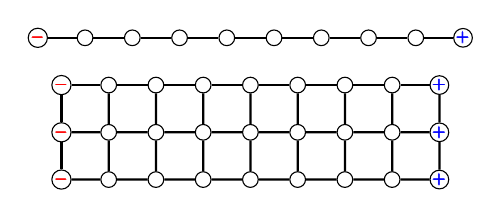
\begin{tikzpicture}[scale=0.6, auto,swap]\tiny
	% First we draw the vertices
	\foreach \pos/\label/\name in {
		{(1.000000,0.000000)/2/},
		{(2.000000,0.000000)/3/},
		{(3.000000,0.000000)/4/},
		{(4.000000,0.000000)/5/},
		{(5.000000,0.000000)/6/},
		{(6.000000,0.000000)/7/},
		{(7.000000,0.000000)/8/},
		{(8.000000,0.000000)/9/}}
	\node[vertex, minimum size = 5pt] (\label) at \pos{};
	
	\foreach \pos/\label/\name in {
		{(9.000000,0.000000)/1/+}}
	\node[positive vertex, synthetic data] (\label) at \pos{$\pmb{\name}$};
	
	\foreach \pos/\label/\name in {
		{(0.000000,0.000000)/0/-}}
	\node[negative vertex,synthetic data] (\label) at \pos{$\pmb{\name}$};
	
	% Connect vertices with edges and draw weights
	\foreach \source/ \dest in {
		1/9,
		0/2,
		2/3,
		3/4,
		4/5,
		5/6,
		6/7,
		7/8,
		8/9}
	\path[edge] (\source) -- (\dest);
	
	% Grid
	% First we draw the vertices
	\foreach \pos/\label/\name in {
		{(1.5,-3)/6/}, {(2.5,-3)/7/}, {(3.5,-3)/8/}, {(4.5,-3)/9/}, {(5.5,-3)/10/}, {(6.5,-3)/11/}, 
		{(7.5,-3)/12/}, {(1.5,-2)/13/}, {(2.5,-2)/14/}, {(3.5,-2)/15/}, {(4.5,-2)/16/}, {(5.5,-2)/17/}, 
		{(6.5,-2)/18/}, {(7.5,-2)/19/}, {(1.5,-1)/20/}, {(2.5,-1)/21/}, {(3.5,-1)/22/}, {(4.5,-1)/23/}, 
		{(5.5,-1)/24/}, {(6.5,-1)/25/}, {(7.5,-1)/26/}}
	\node[vertex, minimum size = 5pt] (\label) at \pos{};
	
	\foreach \pos/\label/\name in {
		{(8.5,-3)/3/+},
		{(8.5,-2)/4/+},
		{(8.5,-1)/5/+}}
	\node[positive vertex, synthetic data] (\label) at \pos{$\pmb{\name}$};
	
	\foreach \pos/\label/\name in {
		{(0.5,-3)/0/-},
		{(0.5,-2)/1/-},
		{(0.5,-1)/2/-}}
	\node[negative vertex,synthetic data] (\label) at \pos{$\pmb{\name}$};
	
	% Connect vertices with edges and draw weights
	\foreach \source/ \dest in {
		0/6, 0/1, 1/13, 1/2, 2/20, 6/7, 6/13, 13/14, 13/20, 20/21, 7/8, 7/14, 14/15, 14/21, 21/22, 
		8/9, 8/15, 15/16, 15/22, 22/23, 9/10, 9/16, 16/17, 16/23, 23/24, 10/11, 10/17, 17/18, 
		17/24, 24/25, 11/12, 11/18, 18/19, 18/25, 25/26, 3/12, 12/19, 4/19, 19/26, 5/26, 3/4, 4/5}
	\path[edge] (\source) -- (\dest);
\end{tikzpicture}
		\caption{Input data}
		\label{fig4a: synthetic data: chain and grid}
	\end{subfigure}
	\hfill
	\begin{subfigure}[b]{0.45\textwidth}
		\centering
		\input{data/synthetic_chain_grid_2}
		\caption{Mincut approach}
		\label{fig4b: synthetic data: chain and grid}
	\end{subfigure}

	\hfill
	
	\begin{subfigure}[b]{0.45\textwidth}
		\centering
		\input{data/synthetic_chain_grid_3}
		\caption{Conventional \\ graphical model}
		\label{fig4c: synthetic data: chain and grid}
	\end{subfigure}
	\hfill
	\begin{subfigure}[b]{0.45\textwidth}
		\centering
		\input{data/synthetic_chain_grid_4}
		\caption{Graphical model \\ using Influence index}
		\label{fig4d: synthetic data: chain and grid}
	\end{subfigure}

	\caption{Inference in synthetic data forms a chain and grid of vertices.}
	\label{fig4: synthetic data: chain and grid}
\end{figure}

Continue to examine more on the case of loopy belief propagation. From section \ref{subsection: influence and loopy belief}, we have known that it is possible to detect when a message is balanced in the sending process immediately with max-sum algorithm. But with loopy belief propagation we need to wait until this process is finished and only be able to examine the equal condition when summing up all the messages on each node. In figure \ref{fig4: synthetic data: circle} we have a circle graph with 14 vertices equally separated, which represents a simplified loop in arbitrary graph. With this form of graph, any combination of 2 edges on upper and lower semicircles is a valid boundary to separate the label groups. The influence index still keeps getting a good separation, figure \ref{fig4d: synthetic data: circle}. 

What we pay attention to is the conventional loop belief propagation in different iterations. The third iteration, figure \ref{fig4b: synthetic data: circle}, messages are on the way to send out on both sides. If we get the results right there, it seems be good. But actually, the messages have not fully spread through the graph yet and this is only a lucky gamble decision that we rarely have. So if we continue the loop, from iteration fourth to seventh, figure \ref{fig4c: synthetic data: circle}, we have a mix of equal messages from both sides then the decision is set to the default value, negative label in this case. Besides, the interesting fact is if we continue the process many times after then, where all the messages have been received all over the graph and resent again, we still have the same result as at seventh iteration. The reason is when the new round of messages starts to resend again, the sum of all the messages sent to one vertex will sum up with the old one. Then more or less, both directions self-balanced themselves, we have the equal results.

\begin{figure}[t!]
	\centering
	\captionsetup[subfigure]{justification=centering}
	\begin{subfigure}[b]{0.24\textwidth}
		\centering
		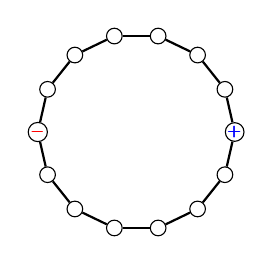
\begin{tikzpicture}[scale=0.25, auto,swap]\tiny
	% First we draw the vertices
	\foreach \pos/\label/\name in {
		{(5.004844339512096,-0.8305813044122092)/2/+},
		{(3.6174490092936677,0.9091574123401482)/3/+},
		{(1.6126046697815721,1.8746395609091184)/4/+},
		{(-0.6126046697815717,1.8746395609091184)/5/-},
		{(-2.617449009293669,0.9091574123401478)/6/-},
		{(-4.004844339512096,-0.830581304412211)/7/-},
		{(-4.004844339512096,-5.16941869558779)/8/-},
		{(-2.6174490092936686,-6.909157412340148)/9/-},
		{(-0.6126046697815686,-7.874639560909118)/10/-},
		{(1.6126046697815752,-7.8746395609091175)/11/+},
		{(3.6174490092936704,-6.909157412340147)/12/+},
		{(5.004844339512097,-5.169418695587788)/13/+}}
	\node[vertex, minimum size = 5pt] (\label) at \pos{};
	
	\foreach \pos/\label/\name in {{(5.5,-3.0)/1/+}}
	\node[positive vertex, synthetic data] (\label) at \pos{$\pmb{\name}$};
	
	\foreach \pos/\label/\name in {{(-4.5,-2.9999999999999996)/0/-}}
	\node[negative vertex,synthetic data] (\label) at \pos{$\pmb{\name}$};
	
	% Connect vertices with edges and draw weights
	\foreach \source/ \dest in {
		2/3,
		3/4,
		4/5,
		5/6,
		6/7,
		8/9,
		9/10,
		10/11,
		11/12,
		12/13,
		0/7,
		0/8,
		1/2,
		1/13}
	\path[edge] (\source) -- (\dest);

\end{tikzpicture}
		\caption{Input data}
		\label{fig4a: synthetic data: circle}
	\end{subfigure}
	\hfill
	\begin{subfigure}[b]{0.24\textwidth}
		\centering
		\input{data/synthetic_circle_2}
		\caption{After 3 iterations}
		\label{fig4b: synthetic data: circle}
	\end{subfigure}
	\hfill
	\begin{subfigure}[b]{0.24\textwidth}
		\centering
		\input{data/synthetic_circle_3}
		\caption{After 7 iterations}
		\label{fig4c: synthetic data: circle}
	\end{subfigure}
	\hfill
	\begin{subfigure}[b]{0.24\textwidth}
		\centering
		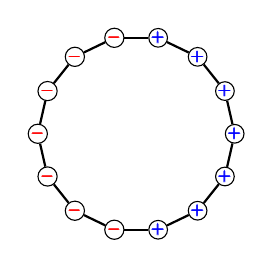
\begin{tikzpicture}[scale=0.25, auto,swap]\tiny
% First we draw the vertices

\foreach \pos/\label/\name in {
	{(5.0,0.0)/1/+},
	{(4.504844339512096,2.1694186955877908)/2/+},
	{(3.1174490092936677,3.9091574123401482)/3/+},
	{(1.1126046697815721,4.874639560909118)/4/+},
	{(1.1126046697815752,-4.8746395609091175)/11/+},
	{(3.1174490092936704,-3.9091574123401474)/12/+},
	{(4.504844339512097,-2.1694186955877877)/13/+}}
\node[positive vertex, synthetic data] (\label) at \pos{$\pmb{\name}$};

\foreach \pos/\label/\name in {
	{(-5.0,6.123233995736766e-16)/0/-},
	{(-1.1126046697815717,4.874639560909118)/5/-},
	{(-3.117449009293669,3.909157412340148)/6/-},
	{(-4.504844339512096,2.169418695587789)/7/-},
	{(-4.504844339512096,-2.16941869558779)/8/-},
	{(-3.1174490092936686,-3.9091574123401482)/9/-},
	{(-1.1126046697815686,-4.874639560909118)/10/-}}
\node[negative vertex,synthetic data] (\label) at \pos{$\pmb{\name}$};

% Connect vertices with edges and draw weights
\foreach \source/ \dest in {
	2/3,
	3/4,
	4/5,
	5/6,
	6/7,
	8/9,
	9/10,
	10/11,
	11/12,
	12/13,
	0/7,
	0/8,
	1/2,
	1/13}
\path[edge] (\source) -- (\dest);

\end{tikzpicture}
		\caption{Influence index}
		\label{fig4d: synthetic data: circle}
	\end{subfigure}
	\caption{Graphical inference in a graph forms a circle of vertices.}
	\label{fig4: synthetic data: circle}
\end{figure}

Lastly, we want to see whether all the things we have made are working on our data distribution assumption. Then we only compare the mincut approach and the graphical model using influence index. In figure \ref{fig4: synthetic data: normal distribution 1}, we have a set of 150 instances made from two normal distributions, $\mathcal{N}(1, 0.6^2)$ for positive and $\mathcal{N}(0, 0.6^2)$ for negative label. The labels were equivalently distributed, with 75 instances including 7 labeled and 68 unlabeled for each. The mincut approach, figure \ref{fig4b: synthetic data: normal distribution 1}, gives us a neat boundary of the separation which hardly divides the center density of each group. The graphical model, figure \ref{fig4c: synthetic data: normal distribution 1}, returns in a tangled boundary. Some measurements of this result are in table \ref{table4: synthetic normal 1}. There is not much to be concluded here, where both models are on track to recognize the boundary and the mixing region is still small.

\begin{figure}[ht!]
	\centering
	\captionsetup[subfigure]{justification=centering}
	\begin{subfigure}[b]{0.31\textwidth}
		\centering
		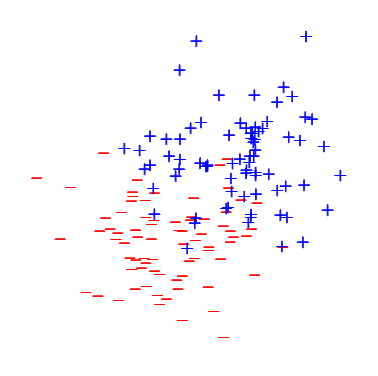
\begin{tikzpicture}[scale=.95, auto,swap]\tiny
			\foreach \pos/\label/\name in {
	{(-0.2225200774229265,-0.32608517245672425)/0/-},
	{(-0.10792698973224357,-0.4322723564304132)/1/-},
	{(-0.43579819547117127,-0.2585310210445544)/2/-},
	{(-0.5098276643544934,-0.06199801779890762)/3/-},
	{(-0.3572219112967324,-0.2901705254124338)/4/-},
	{(-0.24686014357506988,-0.26602094982298574)/5/-},
	{(-0.4122781181743554,-0.41174037627413024)/6/-},
	{(-0.13155402521469958,-0.28265284939268)/7/-},
	{(-0.4013892200821219,0.6194130925380561)/8/-},
	{(-0.038682149507085886,-0.8841269464236071)/9/-},
	{(0.41775279311705266,0.5452836919306788)/10/-},
	{(1.1904429279543804,0.12934373248317083)/11/-},
	{(-0.41432691418775425,0.5020246503499929)/12/-},
	{(-0.14889652692904784,0.1881127108599629)/13/-},
	{(0.9065568090920573,-0.04785238879610198)/14/-},
	{(-0.7610715120240329,0.272872387134225)/15/-},
	{(-0.861744815921591,-0.7708778060573379)/16/-},
	{(1.2616790328054561,0.47283622148673293)/17/-},
	{(0.8823972087062629,0.6771687409090151)/18/-},
	{(0.907386175227952,0.10201909787511977)/19/-},
	{(0.8151941545969827,-1.3229401390732802)/20/-},
	{(-0.3600809460549404,0.11375713002443522)/21/-},
	{(-0.6216368891606755,-0.011828622788958848)/22/-},
	{(0.3886482458977085,0.28519842097236453)/23/-},
	{(0.3739640144981814,0.24875347122026437)/24/-},
	{(-0.7003448143329841,0.12648214505188243)/25/-},
	{(1.1228951823756235,0.03345266618831543)/26/-},
	{(-0.5514053331935688,0.3486980144610941)/27/-},
	{(-0.8405414751795116,0.1008419612116009)/28/-},
	{(-0.22755600921330738,0.5053911984153584)/29/-},
	{(1.2312831692458468,-0.48487307878717706)/30/-},
	{(-0.14880270817774913,-0.004411244360598876)/31/-},
	{(-1.0214210116630718,-0.7200578453405849)/32/-},
	{(-1.682542920343154,0.8120634506562726)/33/-},
	{(0.5197389699875548,0.05911408349384489)/34/-},
	{(0.20624066023889748,-0.6735203793700854)/35/-},
	{(0.2625139378422709,0.1015979089411237)/36/-},
	{(0.8656010941779964,1.059276248934198)/37/-},
	{(0.2826750077050263,-0.07536302179574172)/38/-},
	{(-0.03852398821741344,-0.48227286214472553)/39/-},
	{(-0.28136151536478954,-0.39446624795812957)/40/-},
	{(-0.3313024644512042,0.02157567131174938)/41/-},
	{(0.6100935009885826,-0.6508235109140897)/42/-},
	{(0.052363422936958025,-0.8095424543799895)/43/-},
	{(0.9489381699005437,0.022268071023513282)/44/-},
	{(0.7672476712214347,0.9844728333954431)/45/-},
	{(-0.22182434386182312,0.27963221298609403)/46/-},
	{(0.7766120290084281,-0.2711325015401132)/47/-},
	{(1.0496911867665026,0.5156493304744518)/48/-},
	{(0.8127325614994425,0.16476250666194273)/49/-},
	{(0.2642720963285284,-1.0959841681624427)/50/-},
	{(-1.3666758090695248,-0.00713893417170424)/51/-},
	{(-0.3650145326840327,-0.6730504611209082)/52/-},
	{(-0.3963669255792561,0.5608056869929939)/53/-},
	{(-0.11636929333258177,0.2391172613141169)/54/-},
	{(0.6136753954272933,-0.1613504080046083)/55/-},
	{(-0.0672994614932272,-0.7602379191233869)/56/-},
	{(0.6844367301222299,-0.9740555320476774)/57/-},
	{(0.440420203987672,-0.027778616760857164)/58/-},
	{(0.35719629151702703,-0.30007006274736503)/59/-},
	{(-1.2309475650684873,0.6790650053498698)/60/-},
	{(-0.5994086559093385,0.07646944266252349)/61/-},
	{(0.6197286517310527,-0.11730351058171999)/62/-},
	{(0.21958763515861823,0.10611875050675876)/63/-},
	{(-0.5883992127404697,-0.8308609217808781)/64/-},
	{(-0.3369916105527138,0.7856073817078143)/65/-},
	{(0.5590809097148529,0.26175750577408813)/66/-},
	{(0.4250671397900095,-0.26710133363366423)/67/-},
	{(-0.7875100948809406,1.1398016134428481)/68/-},
	{(0.8521281146228749,0.35319582635900426)/69/-},
	{(0.18895715421089304,-0.5528070760114767)/70/-},
	{(-0.21374246039691278,-0.6394027771092863)/71/-},
	{(1.608251500873829,-0.11895206781670753)/72/-},
	{(0.1722636294332391,0.2207040736771844)/73/-},
	{(-0.10617942514952022,0.6069284647949044)/74/-},
	{(0.2676644060568022,-0.49789415396759906)/75/-}}
\node[negative vertex,synthetic data, draw=none] (\label) at \pos{$\pmb{\name}$};

\foreach \pos/\label/\name in {
	{(1.2326160752073525,1.3234376541212238)/0/+},
	{(1.18126634100516,1.409284058060322)/1/+},
	{(1.283707993678125,1.4311581195421956)/2/+},
	{(1.3989139742981929,1.566047516510241)/3/+},
	{(1.0407760297608515,1.5419064995316616)/4/+},
	{(1.21253590460229,1.2910005600863865)/5/+},
	{(1.2020405154165823,1.40420139366607)/6/+},
	{(1.2392101116906649,1.488783260262376)/7/+},
	{(1.1468176063819597,0.21654487509179432)/8/+},
	{(1.5312777468623744,1.8240008183654495)/9/+},
	{(0.17436518741550844,0.8372839224318885)/10/+},
	{(1.2280673693945807,1.9201724818731143)/11/+},
	{(1.8757259915151439,-0.04678741181443402)/12/+},
	{(-0.167057321969035,0.9789254048224365)/13/+},
	{(0.4304282060887261,0.21051634303401157)/14/+},
	{(1.5753243355301219,0.31572908830356494)/15/+},
	{(1.2445627087126905,0.8831764393154039)/16/+},
	{(1.686471444435738,1.355538138968294)/17/+},
	{(0.9130990594940642,0.8022306819824563)/18/+},
	{(1.6182585102411458,2.0218370328165887)/19/+},
	{(1.9073967440451707,1.6256427879170825)/20/+},
	{(0.22772542588568312,2.2534260011202747)/21/+},
	{(1.733546091697963,1.8984075277942165)/22/+},
	{(0.086893309837621,1.1006261376533484)/23/+},
	{(1.1193119918417844,1.4751070236904238)/24/+},
	{(1.5330537588631583,0.6433292500778514)/25/+},
	{(1.2187062333932948,1.106573406164404)/26/+},
	{(0.37585370102897564,1.4768547457515944)/27/+},
	{(0.5822539624502868,0.9641504363279036)/28/+},
	{(0.5919393941374593,0.9611956521082146)/29/+},
	{(1.0331207611246993,1.0647265591083686)/30/+},
	{(0.9231900767872212,0.6267526504907435)/31/+},
	{(1.8909620118270127,0.718533865252585)/32/+},
	{(0.44507402088776205,0.27094705049763224)/33/+},
	{(1.1164361204277515,0.8765220720175932)/34/+},
	{(1.188133860698395,1.3357523587585303)/35/+},
	{(1.243834254590601,0.8436510348972432)/36/+},
	{(0.7541845778436342,1.9197879281891508)/37/+},
	{(1.0924819941877562,0.5614407575650796)/38/+},
	{(-0.5112210572032863,1.2035737602595757)/39/+},
	{(0.9354912248232083,0.9998490458933262)/40/+},
	{(0.5148907067181836,1.553098215588476)/41/+},
	{(0.22289394571229248,0.9300685317992426)/42/+},
	{(0.45146645247925943,2.6395987932987923)/43/+},
	{(-0.166424060712552,1.3706437709167607)/44/+},
	{(1.1614859876291066,1.0139615483688815)/45/+},
	{(0.2315193712234055,1.0575460834275956)/46/+},
	{(1.3376857163351328,1.4701544761758611)/47/+},
	{(1.9990885932355438,1.598302649463204)/48/+},
	{(0.23366253082156352,1.3289488752291043)/49/+},
	{(1.184440118690655,0.3220342344237722)/50/+},
	{(1.6629785147905967,0.2791844298487036)/51/+},
	{(-0.2392090208428923,0.9283570167288818)/52/+},
	{(0.3294869991553525,-0.1340161763586405)/53/+},
	{(2.157308879298305,1.2301984256501093)/54/+},
	{(0.8890881019229913,1.3825220366540856)/55/+},
	{(-0.3070953393572853,1.1771520885350466)/56/+},
	{(1.4201643493322353,0.860774669113443)/57/+},
	{(1.241098553848087,1.1802593196970175)/58/+},
	{(0.05191678988226933,1.3335726259621392)/59/+},
	{(0.875423132354217,0.41366037925611177)/60/+},
	{(0.8508546465756415,0.40358639942872676)/61/+},
	{(1.9197719023285993,2.7009744997622187)/62/+},
	{(1.1215047479185833,0.912333711433073)/63/+},
	{(0.6025422400785359,0.9841423427079677)/64/+},
	{(-0.1085417345449402,0.331130854509775)/65/+},
	{(2.2059440168255167,0.3782987337349223)/66/+},
	{(1.1678102698129817,1.1043382891263502)/67/+},
	{(1.2485051805588707,0.5931143672895391)/68/+},
	{(1.1791800893144846,0.28317729086784493)/69/+},
	{(-0.12423887021360702,0.6666205633386242)/70/+},
	{(1.5962315209365912,-0.10666504357026674)/71/+},
	{(1.64669426796325,0.7028638139972351)/72/+},
	{(1.8357330498023554,1.3102657969459173)/73/+},
	{(2.3772912710679828,0.8411082602923297)/74/+},
	{(0.5026524784873001,1.0069292252112034)/75/+}}
\node[positive vertex, synthetic data, draw=none] (\label) at \pos{$\pmb{\name}$};

%\draw [red] (0,0) circle [radius=0.6*1.96 ];
%\draw [blue] (1,1) circle [radius=0.6*1.96 ];
		\end{tikzpicture}
		\caption{True data}
		\label{fig4a: synthetic data: normal distribution 1}
	\end{subfigure}
	\hfill
	\begin{subfigure}[b]{0.31\textwidth}
		\centering
		\begin{tikzpicture}[scale=.95, auto,swap]\tiny
			\input{data/synthetic_normal_2}
		\end{tikzpicture}
		\caption{Mincut approach}
		\label{fig4b: synthetic data: normal distribution 1}
	\end{subfigure}
	\hfill
	\begin{subfigure}[b]{0.31\textwidth}
		\centering
		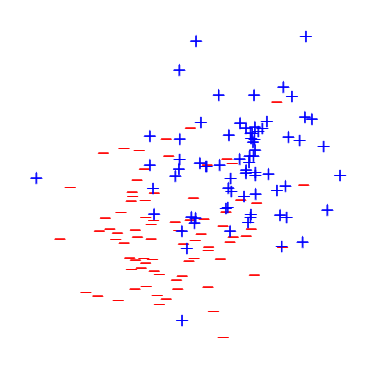
\begin{tikzpicture}[scale=.95, auto,swap]\tiny
		\foreach \pos/\label/\name in {
	{(-0.2225200774229265,-0.32608517245672425)/0/-},
	{(-0.10792698973224357,-0.4322723564304132)/1/-},
	{(-0.43579819547117127,-0.2585310210445544)/2/-},
	{(-0.5098276643544934,-0.06199801779890762)/3/-},
	{(-0.3572219112967324,-0.2901705254124338)/4/-},
	{(-0.24686014357506988,-0.26602094982298574)/5/-},
	{(-0.4122781181743554,-0.41174037627413024)/6/-},
	{(-0.13155402521469958,-0.28265284939268)/7/-},
	{(-0.4013892200821219,0.6194130925380561)/8/-},
	{(-0.038682149507085886,-0.8841269464236071)/9/-},
	{(0.41775279311705266,0.5452836919306788)/10/-},
	{(1.1904429279543804,0.12934373248317083)/11/-},
	{(-0.41432691418775425,0.5020246503499929)/12/-},
	{(-0.14889652692904784,0.1881127108599629)/13/-},
	{(0.9065568090920573,-0.04785238879610198)/14/-},
	{(-0.7610715120240329,0.272872387134225)/15/-},
	{(-0.861744815921591,-0.7708778060573379)/16/-},
	{(1.2616790328054561,0.47283622148673293)/17/-},
	{(0.8151941545969827,-1.3229401390732802)/18/-},
	{(-0.3600809460549404,0.11375713002443522)/19/-},
	{(-0.6216368891606755,-0.011828622788958848)/20/-},
	{(0.3739640144981814,0.24875347122026437)/21/-},
	{(-0.7003448143329841,0.12648214505188243)/22/-},
	{(1.1228951823756235,0.03345266618831543)/23/-},
	{(-0.5514053331935688,0.3486980144610941)/24/-},
	{(-0.8405414751795116,0.1008419612116009)/25/-},
	{(-0.22755600921330738,0.5053911984153584)/26/-},
	{(1.2312831692458468,-0.48487307878717706)/27/-},
	{(-0.14880270817774913,-0.004411244360598876)/28/-},
	{(-1.0214210116630718,-0.7200578453405849)/29/-},
	{(0.5197389699875548,0.05911408349384489)/30/-},
	{(0.20624066023889748,-0.6735203793700854)/31/-},
	{(0.8656010941779964,1.059276248934198)/32/-},
	{(0.2826750077050263,-0.07536302179574172)/33/-},
	{(-0.03852398821741344,-0.48227286214472553)/34/-},
	{(-0.28136151536478954,-0.39446624795812957)/35/-},
	{(-0.3313024644512042,0.02157567131174938)/36/-},
	{(0.6100935009885826,-0.6508235109140897)/37/-},
	{(0.052363422936958025,-0.8095424543799895)/38/-},
	{(0.9489381699005437,0.022268071023513282)/39/-},
	{(-0.22182434386182312,0.27963221298609403)/40/-},
	{(0.7766120290084281,-0.2711325015401132)/41/-},
	{(1.0496911867665026,0.5156493304744518)/42/-},
	{(0.8127325614994425,0.16476250666194273)/43/-},
	{(-1.3666758090695248,-0.00713893417170424)/44/-},
	{(-0.3650145326840327,-0.6730504611209082)/45/-},
	{(-0.3963669255792561,0.5608056869929939)/46/-},
	{(-0.11636929333258177,0.2391172613141169)/47/-},
	{(0.6136753954272933,-0.1613504080046083)/48/-},
	{(-0.0672994614932272,-0.7602379191233869)/49/-},
	{(0.6844367301222299,-0.9740555320476774)/50/-},
	{(0.440420203987672,-0.027778616760857164)/51/-},
	{(0.35719629151702703,-0.30007006274736503)/52/-},
	{(-1.2309475650684873,0.6790650053498698)/53/-},
	{(-0.5994086559093385,0.07646944266252349)/54/-},
	{(0.6197286517310527,-0.11730351058171999)/55/-},
	{(0.21958763515861823,0.10611875050675876)/56/-},
	{(-0.5883992127404697,-0.8308609217808781)/57/-},
	{(-0.3369916105527138,0.7856073817078143)/58/-},
	{(0.5590809097148529,0.26175750577408813)/59/-},
	{(0.4250671397900095,-0.26710133363366423)/60/-},
	{(-0.7875100948809406,1.1398016134428481)/61/-},
	{(0.8521281146228749,0.35319582635900426)/62/-},
	{(0.18895715421089304,-0.5528070760114767)/63/-},
	{(-0.21374246039691278,-0.6394027771092863)/64/-},
	{(1.608251500873829,-0.11895206781670753)/65/-},
	{(0.1722636294332391,0.2207040736771844)/66/-},
	{(-0.10617942514952022,0.6069284647949044)/67/-},
	{(0.2676644060568022,-0.49789415396759906)/68/-},
	{(1.5312777468623744,1.8240008183654495)/69/-},
	{(0.086893309837621,1.1006261376533484)/70/-},
	{(0.37585370102897564,1.4768547457515944)/71/-},
	{(1.8909620118270127,0.718533865252585)/72/-},
	{(-0.5112210572032863,1.2035737602595757)/73/-},
	{(0.9354912248232083,0.9998490458933262)/74/-},
	{(-0.2392090208428923,0.9283570167288818)/75/-},
	{(-0.3070953393572853,1.1771520885350466)/76/-},
	{(0.05191678988226933,1.3335726259621392)/77/-},
	{(0.6025422400785359,0.9841423427079677)/78/-}}
	\node[negative vertex,synthetic data, draw=none] (\label) at \pos{$\pmb{\name}$};
	
	\foreach \pos/\label/\name in {
		{(1.2326160752073525,1.3234376541212238)/0/+},
		{(1.18126634100516,1.409284058060322)/1/+},
		{(1.283707993678125,1.4311581195421956)/2/+},
		{(1.3989139742981929,1.566047516510241)/3/+},
		{(1.0407760297608515,1.5419064995316616)/4/+},
		{(1.21253590460229,1.2910005600863865)/5/+},
		{(1.2020405154165823,1.40420139366607)/6/+},
		{(1.2392101116906649,1.488783260262376)/7/+},
		{(0.8823972087062629,0.6771687409090151)/8/+},
		{(0.907386175227952,0.10201909787511977)/9/+},
		{(0.3886482458977085,0.28519842097236453)/10/+},
		{(-1.682542920343154,0.8120634506562726)/11/+},
		{(0.2625139378422709,0.1015979089411237)/12/+},
		{(0.7672476712214347,0.9844728333954431)/13/+},
		{(0.2642720963285284,-1.0959841681624427)/14/+},
		{(1.1468176063819597,0.21654487509179432)/15/+},
		{(0.17436518741550844,0.8372839224318885)/16/+},
		{(1.2280673693945807,1.9201724818731143)/17/+},
		{(1.8757259915151439,-0.04678741181443402)/18/+},
		{(-0.167057321969035,0.9789254048224365)/19/+},
		{(0.4304282060887261,0.21051634303401157)/20/+},
		{(1.5753243355301219,0.31572908830356494)/21/+},
		{(1.2445627087126905,0.8831764393154039)/22/+},
		{(1.686471444435738,1.355538138968294)/23/+},
		{(0.9130990594940642,0.8022306819824563)/24/+},
		{(1.6182585102411458,2.0218370328165887)/25/+},
		{(1.9073967440451707,1.6256427879170825)/26/+},
		{(0.22772542588568312,2.2534260011202747)/27/+},
		{(1.733546091697963,1.8984075277942165)/28/+},
		{(1.1193119918417844,1.4751070236904238)/29/+},
		{(1.5330537588631583,0.6433292500778514)/30/+},
		{(1.2187062333932948,1.106573406164404)/31/+},
		{(0.5822539624502868,0.9641504363279036)/32/+},
		{(0.5919393941374593,0.9611956521082146)/33/+},
		{(1.0331207611246993,1.0647265591083686)/34/+},
		{(0.9231900767872212,0.6267526504907435)/35/+},
		{(0.44507402088776205,0.27094705049763224)/36/+},
		{(1.1164361204277515,0.8765220720175932)/37/+},
		{(1.188133860698395,1.3357523587585303)/38/+},
		{(1.243834254590601,0.8436510348972432)/39/+},
		{(0.7541845778436342,1.9197879281891508)/40/+},
		{(1.0924819941877562,0.5614407575650796)/41/+},
		{(0.5148907067181836,1.553098215588476)/42/+},
		{(0.22289394571229248,0.9300685317992426)/43/+},
		{(0.45146645247925943,2.6395987932987923)/44/+},
		{(-0.166424060712552,1.3706437709167607)/45/+},
		{(1.1614859876291066,1.0139615483688815)/46/+},
		{(0.2315193712234055,1.0575460834275956)/47/+},
		{(1.3376857163351328,1.4701544761758611)/48/+},
		{(1.9990885932355438,1.598302649463204)/49/+},
		{(0.23366253082156352,1.3289488752291043)/50/+},
		{(1.184440118690655,0.3220342344237722)/51/+},
		{(1.6629785147905967,0.2791844298487036)/52/+},
		{(0.3294869991553525,-0.1340161763586405)/53/+},
		{(2.157308879298305,1.2301984256501093)/54/+},
		{(0.8890881019229913,1.3825220366540856)/55/+},
		{(1.4201643493322353,0.860774669113443)/56/+},
		{(1.241098553848087,1.1802593196970175)/57/+},
		{(0.875423132354217,0.41366037925611177)/58/+},
		{(0.8508546465756415,0.40358639942872676)/59/+},
		{(1.9197719023285993,2.7009744997622187)/60/+},
		{(1.1215047479185833,0.912333711433073)/61/+},
		{(-0.1085417345449402,0.331130854509775)/62/+},
		{(2.2059440168255167,0.3782987337349223)/63/+},
		{(1.1678102698129817,1.1043382891263502)/64/+},
		{(1.2485051805588707,0.5931143672895391)/65/+},
		{(1.1791800893144846,0.28317729086784493)/66/+},
		{(-0.12423887021360702,0.6666205633386242)/67/+},
		{(1.5962315209365912,-0.10666504357026674)/68/+},
		{(1.64669426796325,0.7028638139972351)/69/+},
		{(1.8357330498023554,1.3102657969459173)/70/+},
		{(2.3772912710679828,0.8411082602923297)/71/+},
		{(0.5026524784873001,1.0069292252112034)/72/+}}
		\node[positive vertex, synthetic data, draw=none] (\label) at \pos{$\pmb{\name}$};
		\end{tikzpicture}
		\caption{Graphical model}
		\label{fig4c: synthetic data: normal distribution 1}
	\end{subfigure}
	\caption[Inference outputs on $\mathcal{N}(0, 0.6^2)$ and $\mathcal{N}(1, 0.6^2)$.]{Inference outputs on $\mathcal{N}(0, 0.6^2)$ and $\mathcal{N}(1, 0.6^2)$. 150 instances, 7 labeled and 68 unlabeled for each label.}
	\label{fig4: synthetic data: normal distribution 1}
\end{figure}

\begin{table}[ht!]
	\centering
	\captionsetup{justification=centering}
	\caption{Measurement of inferences on $\mathcal{N}(0, 0.6^2)$ and $\mathcal{N}(1, 0.6^2)$.}
	\makebox[\textwidth][c]{
		\begin{tabular}{ c|ccc|ccc }
			\multirow{2}{*}{Label} & Precision & Recall & F1 & Precision & Recall & F1\\
			\cline{2-7}
			& \multicolumn{3}{c}{\textbf{Mincut approach}} & \multicolumn{3}{c}{\textbf{Graphical model}} \\
			\hline
			
			$-1$ & 0.88 & 0.87 & 0.87 
			& 0.87 & 0.91 & 0.89 \\  % 2
			$+1$ & 0.87 & 0.88 & 0.88 
			& 0.90 & 0.87 & 0.89 \\
			\cline{1-7}
			avg. & 0.88 & 0.88 & 0.87 
			& 0.89 & 0.89 & 0.89 \\
			\hline
	\end{tabular}}
	\label{table4: synthetic normal 1}
\end{table}

Now we twist the two distributions and let them bend more with $\mathcal{N}(0, 0.8^2)$ and $\mathcal{N}(1, 0.8^2)$ on the same set up. The results are in figure \ref{fig4: synthetic data: normal distribution 2}. The true data regions are more chaotic---figure \ref{fig4a: synthetic data: normal distribution 2}---and the mincut approach appears to be shrink to positive region in figure \ref{fig4b: synthetic data: normal distribution 2}. The graphical model using influence index in figure \ref{fig4c: synthetic data: normal distribution 2} seems to have better match in shape of out true data. The estimation indices in table \ref{table4: synthetic normal 2} also shows us the same view of this illustration. If we try to squeeze these distributions more, the objective condition will be violated and the models have nothing to deal with the case.

\begin{figure}[ht!]
	\centering
	\captionsetup[subfigure]{justification=centering}
	\begin{subfigure}[b]{0.31\textwidth}
		\centering
		\begin{tikzpicture}[scale=.9, auto,swap]\tiny
			\input{data/synthetic_normal_4}
		\end{tikzpicture}
		\caption{True data}
		\label{fig4a: synthetic data: normal distribution 2}
	\end{subfigure}
	\hfill
	\begin{subfigure}[b]{0.31\textwidth}
		\centering
		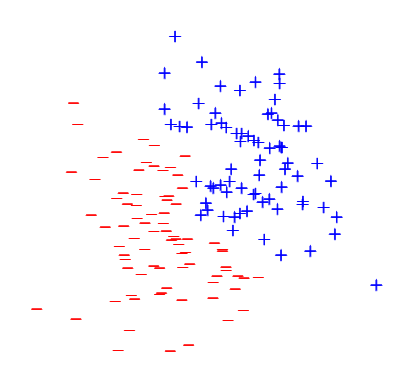
\begin{tikzpicture}[scale=.9, auto,swap]\tiny
			\foreach \pos/\label/\name in {
	{(-0.10238907687639826,-0.4783888445757073)/0/-},
	{(-0.18313250109733775,0.03673512157417608)/1/-},
	{(-0.18390340362848412,-0.4466949708497805)/2/-},
	{(-0.6025671177346985,-0.2962533267692846)/3/-},
	{(-0.3134991566869373,-0.2185453666559894)/4/-},
	{(-0.5868781982577814,-0.3611630050425512)/5/-},
	{(-0.5517052861794693,-0.48109352445605946)/6/-},
	{(-0.36274595223082495,-0.5732683743525453)/7/-},
	{(0.21147692194031587,-0.9266354675625097)/8/-},
	{(1.0792382000401273,-1.0791930565910366)/9/-},
	{(-1.3168947244113198,1.8511443095026412)/10/-},
	{(-0.21617596991035565,0.27359832822245933)/11/-},
	{(1.2902804526784541,-0.6122814982772987)/12/-},
	{(0.7077447870712312,-0.5922510681106375)/13/-},
	{(-0.4245508901433821,0.557787329638177)/14/-},
	{(0.15434650530322402,0.8356911896698439)/15/-},
	{(-0.008116519553535494,0.043030294441896315)/16/-},
	{(-0.4201700916407385,0.21749023762187464)/17/-},
	{(-0.28952526703232645,1.0111221635157133)/18/-},
	{(0.7839935891805094,-0.2378476050527208)/19/-},
	{(-0.5275877690711236,-1.3610164887965275)/20/-},
	{(-0.46154308986926557,-0.06262018614358744)/21/-},
	{(-0.7083671209117792,0.5014448444383899)/22/-},
	{(-0.028336314675048737,0.5290954285357835)/23/-},
	{(-0.07712243325445844,-0.8279192095244231)/24/-},
	{(-0.05564091015894971,0.8943552826488678)/25/-},
	{(0.22313810195107975,-0.4731316511398772)/26/-},
	{(0.6714766752453176,-0.1267593344314163)/27/-},
	{(0.2630521502423141,-0.259106269535963)/28/-},
	{(0.09666971563459716,-0.03284564153480308)/29/-},
	{(0.13036361839994762,0.4235265917112594)/30/-},
	{(-0.5571695808382611,0.42547316023791154)/31/-},
	{(-0.1809124762668233,0.958500742662409)/32/-},
	{(-1.8373635404748183,-1.0548869129023073)/33/-},
	{(-0.6169311834673137,0.5786854174954227)/34/-},
	{(-1.283766622707879,-1.1961102483120996)/35/-},
	{(0.6524929401446484,-0.6819816978766969)/36/-},
	{(0.8636279625345493,-1.2194659855849905)/37/-},
	{(0.8343098748386109,-0.46384130154682934)/38/-},
	{(0.21304752119168602,-0.2710970815667344)/39/-},
	{(-0.03638811130148439,0.29602524796688084)/40/-},
	{(-0.8689058385931022,0.09706177981731856)/41/-},
	{(-1.2584513009365885,1.5440789367364385)/42/-},
	{(-0.7297772153594464,-0.9504105972858788)/43/-},
	{(0.3068715488877769,-1.5618551346526042)/44/-},
	{(-0.6091391953208748,0.11623151880246066)/45/-},
	{(-1.014914703412196,0.767505661724623)/46/-},
	{(-0.6706720270870746,-0.1750173953022809)/47/-},
	{(0.04864815976518914,-1.6533628247056595)/48/-},
	{(-0.30972871390990203,0.15252199531383365)/49/-},
	{(1.0893751468042878,-0.6192006615280468)/50/-},
	{(-0.10305999291596937,-0.8498531100582215)/51/-},
	{(-0.5018893229113084,-0.8682206689684829)/52/-},
	{(-0.43134679163924217,0.4024521071043193)/53/-},
	{(-0.6876359333345086,-1.6453972544632258)/54/-},
	{(-0.4549474445391286,-0.9145131501323016)/55/-},
	{(0.6495952090244139,-0.9056320776933957)/56/-},
	{(0.9635727060734738,-0.7753611467642806)/57/-},
	{(-1.3454703436908027,0.8761278409603881)/58/-},
	{(-0.7119739769613178,1.1593839262759278)/59/-},
	{(0.06531844072577701,-0.08110558822354327)/60/-},
	{(-0.39529646810737007,0.9058660646425671)/61/-},
	{(0.026407328961620014,0.54108851462194)/62/-},
	{(1.004086772952986,-0.5929036478868868)/63/-},
	{(0.12734973522010062,-0.07184397112143093)/64/-},
	{(0.1665825796589503,-0.14856372437380272)/65/-},
	{(0.29152538278189755,-0.06687795032710042)/66/-},
	{(0.0027693665819709112,0.48019576973063727)/67/-},
	{(0.051751610366360556,0.9390961620081331)/68/-},
	{(-0.001223719397573264,-0.7642462113364084)/69/-},
	{(-0.05032289720997052,0.15109829237622963)/70/-},
	{(-0.9008015085004777,1.0817599845359418)/71/-},
	{(0.3227836029876445,-0.4208317637636325)/72/-},
	{(0.7840451740487617,-0.21955555356480438)/73/-},
	{(-0.329517406885943,1.3331824378295842)/74/-},
	{(0.21987740342888695,0.6483726050392908)/75/-},
	{(0.2572457296042314,1.1015880122285093)/76/-},
	{(-0.17613844567278414,1.2473590405697796)/77/-},
	{(0.835815494122677,-0.5121048374465191)/78/-},
	{(-1.066886525790697,0.26806125794820346)/79/-}}
	\node[negative vertex,synthetic data, draw=none] (\label) at \pos{$\pmb{\name}$};

\foreach \pos/\label/\name in {
	{(1.148166034432134,1.3802067580826494)/0/+},
	{(1.4510023725707715,1.2156604137876565)/1/+},
	{(1.037939818706687,1.303356712933553)/2/+},
	{(1.475896085053462,1.7049387098214641)/3/+},
	{(1.2916671122845094,1.2932216893200121)/4/+},
	{(1.228117180099777,1.3180729490232959)/5/+},
	{(1.053619861671351,1.4179005107681184)/6/+},
	{(1.315310173554826,1.0421639362708084)/7/+},
	{(-0.032406874424362624,1.7642947338377746)/8/+},
	{(0.7587700014910338,0.6923390574803013)/9/+},
	{(1.61426953890276,1.2233884859315207)/10/+},
	{(0.47757042312259845,0.26567034369436804)/11/+},
	{(0.5753548346813091,0.3366393343144205)/12/+},
	{(0.6175362755860907,0.6764936503914557)/13/+},
	{(2.023548184621606,-0.24216211662284048)/14/+},
	{(2.956200061070649,-0.7152594248020495)/15/+},
	{(1.3741504914439642,-0.07431360479897861)/16/+},
	{(0.655816056687914,0.64643608449187)/17/+},
	{(0.9554048196403114,0.2428149726555378)/18/+},
	{(1.610862114196291,-0.29460888959141535)/19/+},
	{(0.41463506731475114,0.7399810401865211)/20/+},
	{(2.396007003425717,0.24397314062289308)/21/+},
	{(0.8439126470162045,0.5969686971298395)/22/+},
	{(1.2225668964481315,0.5598864864783097)/23/+},
	{(1.5897690175481756,2.12455492402219)/24/+},
	{(0.11497288567393826,2.7885177668062697)/25/+},
	{(1.0287814155837682,0.29139049026820896)/26/+},
	{(0.9075279705189306,0.9193671480519297)/27/+},
	{(1.3501278324339172,0.4531760483824907)/28/+},
	{(0.9837533286225473,1.4190158691725743)/29/+},
	{(1.8442883682255173,0.8206526652880908)/30/+},
	{(2.2123043475814685,0.37215129640191447)/31/+},
	{(1.1301896499145925,0.32739011885991065)/32/+},
	{(0.5512610497865648,0.43565500341178554)/33/+},
	{(1.9147051474354289,0.41877568902374984)/34/+},
	{(1.4243622643228435,1.691773170252353)/35/+},
	{(1.250300106879437,0.569693452452948)/36/+},
	{(1.5645381890948595,1.6066898548322008)/37/+},
	{(0.7699777252825123,1.568349103760699)/38/+},
	{(1.9202268654685888,0.4597090441952588)/39/+},
	{(1.0310681106672515,2.0236225542006707)/40/+},
	{(-0.03269203241393348,2.273848729889899)/41/+},
	{(1.8596098515047226,1.523784872361227)/42/+},
	{(1.054045987511718,0.6503317329923137)/43/+},
	{(1.4455432976780482,0.49217621685289115)/44/+},
	{(2.1214824206677294,0.9969439040049628)/45/+},
	{(1.5233186532701106,1.8996493500556257)/46/+},
	{(0.44798626833422506,1.8424189214572309)/47/+},
	{(0.49497020966134975,2.4312582150143043)/48/+},
	{(0.885538130521679,0.7436524982643853)/49/+},
	{(1.2501373916840008,2.146686827574145)/50/+},
	{(0.6270578451089794,1.5443546790519758)/51/+},
	{(1.5600467347588234,0.3506123338510809)/52/+},
	{(1.5898398531930336,1.2407401757081413)/53/+},
	{(0.7557194054173584,2.089957216381004)/54/+},
	{(0.1784350926172289,1.519769163973463)/55/+},
	{(0.8378253288109326,1.5053422122018638)/56/+},
	{(1.6197976705241475,0.6627146849333687)/57/+},
	{(0.7986207099565037,0.25103294003430987)/58/+},
	{(0.9313397381579959,0.04997911966769786)/59/+},
	{(2.3704014074550814,-0.001923193588837524)/60/+},
	{(0.2835576903546153,1.511827033296007)/61/+},
	{(1.5872051686205808,2.259223488954144)/62/+},
	{(1.6519346556002121,1.5341996074338324)/63/+},
	{(2.314971427294611,0.7487372059087024)/64/+},
	{(1.6239008104111146,1.2197851629861503)/65/+},
	{(1.705720138451762,1.002988764032511)/66/+},
	{(0.6832656245729141,1.711907982878574)/67/+},
	{(1.9653142462314888,1.5226801732736357)/68/+},
	{(1.6664535426343339,0.9168627207128499)/69/+},
	{(0.05560471491676211,1.5464034554699326)/70/+},
	{(1.3035831153302326,0.8328788493432966)/71/+}}
	\node[positive vertex, synthetic data, draw=none] (\label) at \pos{$\pmb{\name}$};

%\draw [red] (0,0) circle [radius=0.6*1.96 ];
%\draw [blue] (1,1) circle [radius=0.6*1.96 ];
		\end{tikzpicture}
		\caption{Mincut approach}
		\label{fig4b: synthetic data: normal distribution 2}
	\end{subfigure}
	\hfill
	\begin{subfigure}[b]{0.31\textwidth}
		\centering
		\begin{tikzpicture}[scale=.9, auto,swap]\tiny
			\begin{tikzpicture}[scale=.9, auto,swap]\tiny
% First we draw the vertices

\foreach \pos/\label/\name in {
	{(-0.10238907687639826,-0.4783888445757073)/0/-},
	{(-0.18313250109733775,0.03673512157417608)/1/-},
	{(-0.18390340362848412,-0.4466949708497805)/2/-},
	{(-0.6025671177346985,-0.2962533267692846)/3/-},
	{(-0.3134991566869373,-0.2185453666559894)/4/-},
	{(-0.5868781982577814,-0.3611630050425512)/5/-},
	{(-0.5517052861794693,-0.48109352445605946)/6/-},
	{(-0.36274595223082495,-0.5732683743525453)/7/-},
	{(0.21147692194031587,-0.9266354675625097)/8/-},
	{(-1.3168947244113198,1.8511443095026412)/9/-},
	{(-0.21617596991035565,0.27359832822245933)/10/-},
	{(-0.032406874424362624,1.7642947338377746)/11/-},
	{(1.2902804526784541,-0.6122814982772987)/12/-},
	{(0.7077447870712312,-0.5922510681106375)/13/-},
	{(0.7587700014910338,0.6923390574803013)/14/-},
	{(-0.4245508901433821,0.557787329638177)/15/-},
	{(0.15434650530322402,0.8356911896698439)/16/-},
	{(1.61426953890276,1.2233884859315207)/17/-},
	{(-0.008116519553535494,0.043030294441896315)/18/-},
	{(-0.4201700916407385,0.21749023762187464)/19/-},
	{(0.7839935891805094,-0.2378476050527208)/20/-},
	{(-0.5275877690711236,-1.3610164887965275)/21/-},
	{(-0.46154308986926557,-0.06262018614358744)/22/-},
	{(-0.7083671209117792,0.5014448444383899)/23/-},
	{(-0.028336314675048737,0.5290954285357835)/24/-},
	{(0.22313810195107975,-0.4731316511398772)/25/-},
	{(0.6714766752453176,-0.1267593344314163)/26/-},
	{(0.2630521502423141,-0.259106269535963)/27/-},
	{(0.09666971563459716,-0.03284564153480308)/28/-},
	{(0.13036361839994762,0.4235265917112594)/29/-},
	{(0.6175362755860907,0.6764936503914557)/30/-},
	{(-0.5571695808382611,0.42547316023791154)/31/-},
	{(2.023548184621606,-0.24216211662284048)/32/-},
	{(-0.1809124762668233,0.958500742662409)/33/-},
	{(-1.8373635404748183,-1.0548869129023073)/34/-},
	{(-0.6169311834673137,0.5786854174954227)/35/-},
	{(-1.283766622707879,-1.1961102483120996)/36/-},
	{(0.6524929401446484,-0.6819816978766969)/37/-},
	{(0.8636279625345493,-1.2194659855849905)/38/-},
	{(0.8343098748386109,-0.46384130154682934)/39/-},
	{(0.21304752119168602,-0.2710970815667344)/40/-},
	{(-0.03638811130148439,0.29602524796688084)/41/-},
	{(-0.8689058385931022,0.09706177981731856)/42/-},
	{(-1.2584513009365885,1.5440789367364385)/43/-},
	{(-0.7297772153594464,-0.9504105972858788)/44/-},
	{(0.3068715488877769,-1.5618551346526042)/45/-},
	{(-0.6091391953208748,0.11623151880246066)/46/-},
	{(-1.014914703412196,0.767505661724623)/47/-},
	{(1.3741504914439642,-0.07431360479897861)/48/-},
	{(0.04864815976518914,-1.6533628247056595)/49/-},
	{(0.655816056687914,0.64643608449187)/50/-},
	{(-0.30972871390990203,0.15252199531383365)/51/-},
	{(1.0893751468042878,-0.6192006615280468)/52/-},
	{(-0.10305999291596937,-0.8498531100582215)/53/-},
	{(-0.5018893229113084,-0.8682206689684829)/54/-},
	{(-0.43134679163924217,0.4024521071043193)/55/-},
	{(0.9554048196403114,0.2428149726555378)/56/-},
	{(-0.6876359333345086,-1.6453972544632258)/57/-},
	{(1.610862114196291,-0.29460888959141535)/58/-},
	{(-0.4549474445391286,-0.9145131501323016)/59/-},
	{(0.6495952090244139,-0.9056320776933957)/60/-},
	{(0.9635727060734738,-0.7753611467642806)/61/-},
	{(0.41463506731475114,0.7399810401865211)/62/-},
	{(-1.3454703436908027,0.8761278409603881)/63/-},
	{(-0.7119739769613178,1.1593839262759278)/64/-},
	{(0.8439126470162045,0.5969686971298395)/65/-},
	{(-0.39529646810737007,0.9058660646425671)/66/-},
	{(1.8442883682255173,0.8206526652880908)/67/-},
	{(0.12734973522010062,-0.07184397112143093)/68/-},
	{(1.9147051474354289,0.41877568902374984)/69/-},
	{(0.051751610366360556,0.9390961620081331)/70/-},
	{(2.1214824206677294,0.9969439040049628)/71/-},
	{(0.44798626833422506,1.8424189214572309)/72/-},
	{(0.885538130521679,0.7436524982643853)/73/-},
	{(1.5898398531930336,1.2407401757081413)/74/-},
	{(0.7557194054173584,2.089957216381004)/75/-},
	{(0.1784350926172289,1.519769163973463)/76/-},
	{(0.9313397381579959,0.04997911966769786)/77/-},
	{(2.314971427294611,0.7487372059087024)/78/-},
	{(0.835815494122677,-0.5121048374465191)/79/-}}
	\node[negative vertex,synthetic data, draw=none] (\label) at \pos{$\pmb{\name}$};

\foreach \pos/\label/\name in {
	{(1.148166034432134,1.3802067580826494)/0/+},
	{(1.4510023725707715,1.2156604137876565)/1/+},
	{(1.037939818706687,1.303356712933553)/2/+},
	{(1.475896085053462,1.7049387098214641)/3/+},
	{(1.2916671122845094,1.2932216893200121)/4/+},
	{(1.228117180099777,1.3180729490232959)/5/+},
	{(1.053619861671351,1.4179005107681184)/6/+},
	{(1.315310173554826,1.0421639362708084)/7/+},
	{(1.0792382000401273,-1.0791930565910366)/8/+},
	{(-0.28952526703232645,1.0111221635157133)/9/+},
	{(0.47757042312259845,0.26567034369436804)/10/+},
	{(0.5753548346813091,0.3366393343144205)/11/+},
	{(-0.07712243325445844,-0.8279192095244231)/12/+},
	{(-0.05564091015894971,0.8943552826488678)/13/+},
	{(2.956200061070649,-0.7152594248020495)/14/+},
	{(-0.6706720270870746,-0.1750173953022809)/15/+},
	{(2.396007003425717,0.24397314062289308)/16/+},
	{(0.06531844072577701,-0.08110558822354327)/17/+},
	{(1.2225668964481315,0.5598864864783097)/18/+},
	{(1.5897690175481756,2.12455492402219)/19/+},
	{(0.11497288567393826,2.7885177668062697)/20/+},
	{(1.0287814155837682,0.29139049026820896)/21/+},
	{(0.9075279705189306,0.9193671480519297)/22/+},
	{(0.026407328961620014,0.54108851462194)/23/+},
	{(1.004086772952986,-0.5929036478868868)/24/+},
	{(1.3501278324339172,0.4531760483824907)/25/+},
	{(0.9837533286225473,1.4190158691725743)/26/+},
	{(2.2123043475814685,0.37215129640191447)/27/+},
	{(1.1301896499145925,0.32739011885991065)/28/+},
	{(0.5512610497865648,0.43565500341178554)/29/+},
	{(0.1665825796589503,-0.14856372437380272)/30/+},
	{(1.4243622643228435,1.691773170252353)/31/+},
	{(1.250300106879437,0.569693452452948)/32/+},
	{(1.5645381890948595,1.6066898548322008)/33/+},
	{(0.7699777252825123,1.568349103760699)/34/+},
	{(0.29152538278189755,-0.06687795032710042)/35/+},
	{(1.9202268654685888,0.4597090441952588)/36/+},
	{(1.0310681106672515,2.0236225542006707)/37/+},
	{(-0.03269203241393348,2.273848729889899)/38/+},
	{(0.0027693665819709112,0.48019576973063727)/39/+},
	{(1.8596098515047226,1.523784872361227)/40/+},
	{(1.054045987511718,0.6503317329923137)/41/+},
	{(1.4455432976780482,0.49217621685289115)/42/+},
	{(1.5233186532701106,1.8996493500556257)/43/+},
	{(-0.001223719397573264,-0.7642462113364084)/44/+},
	{(0.49497020966134975,2.4312582150143043)/45/+},
	{(-0.05032289720997052,0.15109829237622963)/46/+},
	{(1.2501373916840008,2.146686827574145)/47/+},
	{(-0.9008015085004777,1.0817599845359418)/48/+},
	{(0.3227836029876445,-0.4208317637636325)/49/+},
	{(0.6270578451089794,1.5443546790519758)/50/+},
	{(1.5600467347588234,0.3506123338510809)/51/+},
	{(0.8378253288109326,1.5053422122018638)/52/+},
	{(0.7840451740487617,-0.21955555356480438)/53/+},
	{(1.6197976705241475,0.6627146849333687)/54/+},
	{(0.7986207099565037,0.25103294003430987)/55/+},
	{(2.3704014074550814,-0.001923193588837524)/56/+},
	{(0.2835576903546153,1.511827033296007)/57/+},
	{(-0.329517406885943,1.3331824378295842)/58/+},
	{(1.5872051686205808,2.259223488954144)/59/+},
	{(1.6519346556002121,1.5341996074338324)/60/+},
	{(1.6239008104111146,1.2197851629861503)/61/+},
	{(1.705720138451762,1.002988764032511)/62/+},
	{(0.21987740342888695,0.6483726050392908)/63/+},
	{(0.2572457296042314,1.1015880122285093)/64/+},
	{(0.6832656245729141,1.711907982878574)/65/+},
	{(1.9653142462314888,1.5226801732736357)/66/+},
	{(1.6664535426343339,0.9168627207128499)/67/+},
	{(-0.17613844567278414,1.2473590405697796)/68/+},
	{(0.05560471491676211,1.5464034554699326)/69/+},
	{(-1.066886525790697,0.26806125794820346)/70/+},
	{(1.3035831153302326,0.8328788493432966)/71/+}}
	\node[positive vertex, synthetic data, draw=none] (\label) at \pos{$\pmb{\name}$};

%\draw [red] (0,0) circle [radius=0.6*1.96 ];
%\draw [blue] (1,1) circle [radius=0.6*1.96 ];

\end{tikzpicture}
		\end{tikzpicture}
		\caption{Graphical model}
		\label{fig4c: synthetic data: normal distribution 2}
	\end{subfigure}
	\caption[Inference outputs on $\mathcal{N}(0, 0.8^2)$ and $\mathcal{N}(1, 0.8^2)$.]{Inference outputs on $\mathcal{N}(0, 0.8^2)$ and $\mathcal{N}(1, 0.8^2)$. 150 instances, 7 labeled and 68 unlabeled for each label.}
	\label{fig4: synthetic data: normal distribution 2}
\end{figure}

\begin{table}[ht!]
	\centering
	\captionsetup{justification=centering}
	\caption{Measurement of inferences on $\mathcal{N}(0, 0.8^2)$ and $\mathcal{N}(1, 0.8^2)$.}
	\makebox[\textwidth][c]{
		\begin{tabular}{ c|ccc|ccc }
			\multirow{2}{*}{Label} & Precision & Recall & F1 & Precision & Recall & F1\\
			\cline{2-7}
			& \multicolumn{3}{c}{\textbf{Mincut approach}} & \multicolumn{3}{c}{\textbf{Graphical model}} \\
			\hline
			
			$-1$ & 0.76 & 0.80 & 0.78
			& 0.82 & 0.87 & 0.85 \\  % 2
			$+1$ & 0.79 & 0.75 & 0.77
			& 0.86 & 0.82 & 0.84 \\
			\cline{1-7}
			avg. & 0.78 & 0.78 & 0.78 
			& 0.84 & 0.84 & 0.84 \\
			\hline
	\end{tabular}}
	\label{table4: synthetic normal 2}
\end{table}

To give more demonstrations for graphical models is a reasonable replacement for the mincut approach, and to examine our graph-based models in practical data, the next section gives us the experimental results taken on some common data sets.

%%%%%
\section{Experimental Results}
In this section, we evaluate our graph-based models by both views of application: transductive semi-supervised learning when predicting unlabeled data in section \ref{subsection: exp ssl} and in compare with some supervised learning in section \ref{subsection: exp sl}. 

In all data cases, we continue to use the splitting ratio of labeled and unlabeled data on the train set from section \ref{sec2: exp results}. Because the learning methods are transductive, we entirely treat the data set as train data. Then, using a split we separate the data set into labeled and unlabeled sets. Figure \ref{fig3: data preparing process} illustrates this overall splitting process.
\begin{figure}[ht!]
	\centering
	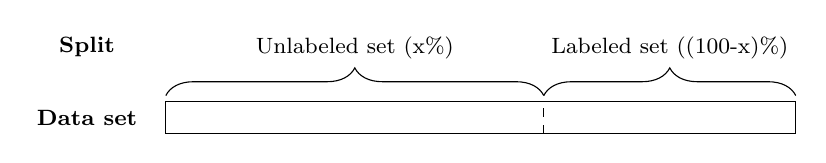
\begin{tikzpicture}[scale=0.8]
	\draw (0,0) rectangle (10,0.5) node[midway]{};
	\draw[dashed] (6,0) -- (6,0.5);
	
	\draw node[draw=none, xshift=-1cm, yshift=1.1cm, align=right] {\footnotesize \textbf{Split}};
	\draw node[draw=none, xshift=-1cm, yshift=.2cm] {\textbf{\footnotesize Data set}};
	
	\draw [decorate,decoration={brace,amplitude=10pt}, yshift=.1cm]
	(0,.5) -- (6,.5) node [black,midway,yshift=0.6cm] {\footnotesize Unlabeled set (x\%)};
	\draw [decorate,decoration={brace,amplitude=10pt}, yshift=.1cm]
	(6,.5) -- (10,.5) node [black,midway,yshift=0.6cm] {\footnotesize Labeled set ((100-x)\%)};
	
	\end{tikzpicture}
	\caption{The split-x on a specific data cases for graph-based models.}
	\label{fig3: data preparing process}
\end{figure}

Continuing with similarity measurement, there were 3 types of function in used including Euclidean, cosine and Gaussian kernel using default bandwidth equals to number of features. As graph sparsity methods are described in previous section \ref{section3: Graph Construction}, the experiments constructed three different kinds of graph with modifications
\begin{description}
	\item[kNN graph:] Search for the most k similar vertices. The search range for k was $[1, 10]$. In the case of sparse graph, it is possible to have a component with all data that are unlabeled. We bypass this problem by constraining that there must be at least one labeled data in neighbor search.
	
	\item[MST tree:] Construct a maximum spanning tree on $\mathcal{G}$. The greedy Prim algorithm \parencite{6773228} was implemented. %The complexity of this algorithm is $\mathcal{O}(|E| log(n))$.
	
	\item[kNN-MST graph:] Construct a kNN graph first, then find a MST tree for each component of this kNN graph.
\end{description}

We only present the inference results of the mincut approach and graphical model using the influence index---we now short its name to the graphical model. The reason is that the conventional graphical model for our problem is not a completed one, it only works on a tree. Moreover, as has been shown in previous section, it does not have the adaption to our data assumption. Hence more or less, even with only the tree construction, it is no better than the mincut approach. Besides that, we have conducted the evaluation on the randomized mincut approach in section \ref{section3: mincut approach}, and it did not turn well either. The complete output of experiments and more details about the data resources and experiment reproduction are described in appendix \ref{appx: Experiments Resources}.

%%%%%%%%%%%%%%%%%%%%%%%%%%%%%%%%%%%%%%%%
\subsection{Semi-Supervised Evaluation}
\label{subsection: exp ssl}

The semi-supervised evaluation considers the ability of models to predict the unlabeled data in various scaling size of unlabeled set. The model learns all data instances and predicts the label for the unlabeled set. For each experimental data set, the experiment ran on 3 splits, split-70, split-90 and split-97, and the result was an average of 5-folds cross validation. In total we have 3 split sizes and 5-folds cross validation, $(3\times5) = 15$ evaluations for each model configuration.

\subsubsection*{Abalone and Digit data}
Abalone data was set on a binary task that determines the age range of abalone is $[5, 9]$ or $[10, 15]$ with 3842 instances, 7 features. The Digit data task was to clarify whether an $8\times8$ digit image---64 features---is odd or even digit with 1797 instances. Both data were set on Euclidean similarity and Gaussian kernel with all three graph sparsity functions. Here we have 2 data cases, 2 similarity measurements, 3 graph types, $(2 \times 2 \times 3) = 12$ configurations. 

The result of Abalone data using Euclidean similarity is in table \ref{table4: exp ssl abalone}, the trend is similar with Gaussian kernel. At first glance, we can observe that the mincut approach has the equivalent or better performance in case of split-70, especially with kNN graph. Here the kNN graph also illustrates its lead over MST and kNN-MST graphs. The situation changes when we significantly shrink the labeled size with split-97. Inform that the split-70 specifies that the unlabeled size is about 2 times bigger than the labeled one, while the split-97 means the difference is now about 32 times. In this case, the graphical model using kNN graph outperforms the mincut approach. Also the MST and kNN-MST graphs take off the gap with kNN graph and the results are nearly the same on both inference models.

We will continue with Digit data. In the same way, table \ref{table4: exp ssl digit} shows the results of Digit data with Euclidean similarity.  Take a look at graphical model, we may allegedly observe that, in kNN graph, the loopy belief propagation could not be converged on a group of vertices. This pushes the recall on positive label high up, but downgrades precision significantly compared with the mincut approach, and the reverse situation is applied to negative label. The equivalent outputs are held on MST and kNN-MST graph.

\subsubsection*{20Newsgroups data}
The 20Newsgroups data was constructed with tf-idf vectorization, the size of vocabulary reduced to 600 words by sum of tf-idf. The original data set consists of many groups of different topic labels. Here we set up an experiment between comp versus rec groups, in 8870 instances. We only use cosine similarity measurement with 3 types of graph construction. Thus we have 1 classifier, 1 similarity measurement, 3 graph types, $(1 \times 1 \times 3) = 3$ configurations.

The results are in table \ref{table4: exp ssl news}. This time, the performance of kNN graph prevails the other two graphs in both mincut approach and graphical model. With split-70 and split-90, we do not have much to say. But there in split-97, the mincut approach has fallen to a degenerate solution when vastly going for the negative label. If we solely examine the MST and kNN-MST graphs, the slightly better outcome comes from the mincut approach.  
% The situation is the same in comp versus sci task. Now we only examine the split-97 of this classifier in table \ref{table4: exp ssl news2 0.97}

%%%%%%%%%%%%%%%%%%%%%%%%%%%%%%%%%%%%%%%%
\subsection{Supervised Evaluation}
\label{subsection: exp sl}

In the same data setup of semi-supervised evaluation, for each data set, we added-in two supervised models including Logistic Regression and Support Vector Machines (SVM, using RBF kernel, $\gamma=\frac{1}{\#features}$) to predict the unlabeled data. In total we have 2 added supervised models, 3 split sizes and 5-folds cross validation, $(2 \times 3 \times 5) = 30$ additional evaluations for each data case. 

From the previous evaluation, we would claim the presume that with the carefully selected graph construction for a specific data, the graphical model can have the advantage over the mincut approach. Therefore, in this section, we only compare the supervised model with the graphical model. We also assume that we already evaluated the graph construction methods and utilize the best one here. 

In table \ref{table4: exp sl abalone} we have the comparison on Abalone data, the graphical model works on Euclidean kNN graph. The table starts with the split-70 where we have merely equivalent outcomes. Then go down with the split-90 and split-97, the logistic regression has the most recognizable downgrade. The graphical model has its solid performance and states first on split-97 in comparison with the other two. A similar result for Digit data is in table \ref{table4: exp sl digit} with Euclidean kNN-MST graph for graphical model. But at this time, the logistic regression has been downed from the beginning. Finally, the result of 20newsgroup data is in table \ref{table4: exp sl news}, graphical model utilizes cosine kNN graph. The supervised keeps its benefits in split-70 and split-90. In split-97, SVM has fallen into a degenerate trap when predicting most of the label for negative. It is the same situation with kNN graph of the mincut approach for this data case.

\pagebreak

\begin{table}[t!]
	\centering
	\captionsetup{justification=centering}
	\caption{Semi-supervised evaluation, Abalone data using Euclidean similarity.}
	\label{table4: exp ssl abalone}
	\makebox[\textwidth][c]{
		\begin{tabular}{ c|c|ccc|ccc }
			\multirow{2}{*}{Graph type} & \multirow{2}{*}{Label} & Precision & Recall & F1 & Precision & Recall & F1\\
			\cline{3-8}
			&& \multicolumn{3}{c}{\textbf{Mincut approach}} & \multicolumn{3}{c}{\textbf{Graphical model}} \\
			\hline
			
			\multicolumn{2}{c}{} & \multicolumn{6}{c}{Split-70, labeled:unlabeled = 1152:2690}\\
			
			\hline
			\multirow{3}{*}{kNN}
			& $-1$ & 0.73 & 0.79 & 0.76 & 0.69 & 0.79 & 0.73 \\
			& $+1$ & 0.80 & 0.74 & 0.76 & 0.78 & 0.67 & 0.72 \\
			\cline{2-8}
			& avg. & 0.76 & 0.76 & 0.76 & 0.74 & 0.73 & 0.73 \\
			\hline
			\multirow{3}{*}{MST} 
			& $-1$ & 0.72 & 0.71 & 0.71 & 0.72 & 0.71 & 0.71 \\
			& $+1$ & 0.74 & 0.75 & 0.74 & 0.74 & 0.75 & 0.74 \\
			\cline{2-8}
			& avg. & 0.73 & 0.73 & 0.73 & 0.73 & 0.73 & 0.73 \\
			\hline
			\multirow{3}{*}{kNN-MST} 
			& $-1$ & 0.71 & 0.70 & 0.70 & 0.71 & 0.70 & 0.70 \\
			& $+1$ & 0.73 & 0.75 & 0.74 & 0.73 & 0.75 & 0.74 \\
			\cline{2-8}
			& avg. & 0.72 & 0.72 & 0.72 & 0.72 & 0.72 & 0.72 \\
			\hline
			
			\multicolumn{2}{c}{} & \multicolumn{6}{c}{Split-90, labeled:unlabeled = 384:3458}\\
			
			\hline
			\multirow{3}{*}{kNN} 
			& $-1$ & 0.71 & 0.74 & 0.72 & 0.71 & 0.70 & 0.70 \\
			& $+1$ & 0.76 & 0.73 & 0.74 & 0.73 & 0.74 & 0.74 \\
			\cline{2-8}
			& avg. & 0.73 & 0.73 & 0.73 & 0.72 & 0.72 & 0.72 \\
			\hline
			\multirow{3}{*}{MST} 
			& $-1$ & 0.70 & 0.67 & 0.68 & 0.70 & 0.67 & 0.68 \\
			& $+1$ & 0.71 & 0.74 & 0.73 & 0.71 & 0.74 & 0.73 \\
			\cline{2-8}
			& avg. & 0.71 & 0.70 & 0.70 & 0.71 & 0.70 & 0.70 \\
			\hline
			\multirow{3}{*}{kNN-MST} 
			& $-1$ & 0.69 & 0.66 & 0.67 & 0.69 & 0.66 & 0.67 \\
			& $+1$ & 0.71 & 0.73 & 0.72  & 0.71 & 0.73 & 0.72 \\ 
			\cline{2-8}
			& avg. & 0.70 & 0.69 & 0.69 & 0.70 & 0.69 & 0.69 \\
			\hline
			
			\multicolumn{2}{c}{} & \multicolumn{6}{c}{Split-97, labeled:unlabeled = 115:3727}\\
			
			\hline
			\multirow{3}{*}{kNN} 
			& $-1$ & 0.69 & 0.66 & 0.67 & 0.69 & 0.73 & 0.71 \\
			& $+1$ & 0.70 & 0.73 & 0.72 & 0.74 & 0.71 & 0.72 \\
			\cline{2-8}
			& avg. & 0.69 & 0.69 & 0.69 & 0.72 & 0.72 & 0.72 \\
			\hline
			\multirow{3}{*}{MST} 
			& $-1$ & 0.70 & 0.64 & 0.67 & 0.70 & 0.64 & 0.67 \\
			& $+1$ & 0.70 & 0.75 & 0.72 & 0.70 & 0.75 & 0.72 \\
			\cline{2-8}
			& avg. & 0.70 & 0.70 & 0.70 & 0.70 & 0.70 & 0.70 \\
			\hline
			\multirow{3}{*}{kNN-MST} 
			& $-1$ & 0.69 & 0.64 & 0.66 & 0.69 & 0.64 & 0.66 \\
			& $+1$ & 0.70 & 0.73 & 0.71 & 0.70 & 0.73 & 0.71 \\
			\cline{2-8}
			& avg. & 0.69 & 0.69 & 0.69 & 0.69 & 0.69 & 0.69 \\
			\hline
	\end{tabular}}
\end{table}

\begin{table}[t!]
	\centering
	\captionsetup{justification=centering}
	\caption{Semi-supervised evaluation, Digit data using Euclidean similarity.}
	\label{table4: exp ssl digit}
	\makebox[\textwidth][c]{
		\begin{tabular}{ c|c|ccc|ccc }
			\multirow{2}{*}{Graph type} & \multirow{2}{*}{Label} & Precision & Recall & F1 & Precision & Recall & F1\\
			\cline{3-8}
			&& \multicolumn{3}{c}{\textbf{Mincut approach}} & \multicolumn{3}{c}{\textbf{Graphical model}} \\
			\hline
			
			\multicolumn{2}{c}{} & \multicolumn{6}{c}{Split-70,  data number labeled-unlabeled : 539-1258}\\
			
			\hline
			\multirow{3}{*}{kNN} 
			& $-1$ & 1.00 & 0.99 & 0.99 & 1.00 & 0.99 & 0.99 \\
			& $+1$ & 0.99 & 1.00 & 0.99 & 0.99 & 1.00 & 0.99 \\
			\cline{2-8}
			& avg. & 0.99 & 0.99 & 0.99 & 0.99 & 0.99 & 0.99 \\
			\hline
			\multirow{3}{*}{MST} 
			& $-1$ & 1.00 & 0.99 & 0.99 & 1.00 & 0.99 & 0.99 \\
			& $+1$ & 0.99 & 1.00 & 0.99 & 0.99 & 1.00 & 0.99 \\
			\cline{2-8}
			& avg. & 0.99 & 0.99 & 0.99 & 0.99 & 0.99 & 0.99 \\
			\hline
			\multirow{3}{*}{kNN-MST} 
			& $-1$ & 1.00 & 0.99 & 0.99 & 1.00 & 0.99 & 0.99 \\
			& $+1$ & 0.99 & 1.00 & 0.99 & 0.99 & 1.00 & 0.99 \\
			\cline{2-8}
			& avg. & 0.99 & 0.99 & 0.99 & 0.99 & 0.99 & 0.99 \\
			\hline
			
			\multicolumn{2}{c}{} & \multicolumn{6}{c}{Split-90,  data number labeled-unlabeled : 179-1618}\\
			
			\hline
			\multirow{3}{*}{kNN} 
			& $-1$ & 0.98 & 0.98 & 0.98 & 0.93 & 0.84 & 0.88 \\
			& $+1$ & 0.98 & 0.98 & 0.98 & 0.86 & 0.94 & 0.90 \\
			\cline{2-8}
			& avg. & 0.98 & 0.98 & 0.98 & 0.89 & 0.89 & 0.89 \\
			\hline
			\multirow{3}{*}{MST} 
			& $-1$ & 0.99 & 0.98 & 0.99 & 0.99 & 0.98 & 0.99 \\
			& $+1$ & 0.99 & 0.99 & 0.99 & 0.99 & 0.99 & 0.99 \\
			\cline{2-8}
			& avg. & 0.99 & 0.99 & 0.99 & 0.99 & 0.99 & 0.99 \\
			\hline
			\multirow{3}{*}{kNN-MST} 
			& $-1$ & 0.99 & 0.98 & 0.99 & 0.99 & 0.98 & 0.99 \\
			& $+1$ & 0.98 & 0.99 & 0.99 & 0.98 & 0.99 & 0.99 \\ 
			\cline{2-8}
			& avg. & 0.99 & 0.99 & 0.99 & 0.99 & 0.99 & 0.99 \\
			\hline
			
			\multicolumn{2}{c}{} & \multicolumn{6}{c}{Split-97,  data number labeled-unlabeled : 53-1744}\\
			
			\hline
			\multirow{3}{*}{kNN} 
			& $-1$ & 0.93 & 0.97 & 0.95 & 0.91 & 0.77 & 0.83 \\
			& $+1$ & 0.97 & 0.93 & 0.95 & 0.80 & 0.92 & 0.86 \\
			\cline{2-8}
			& avg. & 0.95 & 0.95 & 0.95 & 0.86 & 0.84 & 0.84 \\
			\hline
			\multirow{3}{*}{MST} 
			& $-1$ & 0.90 & 0.98 & 0.93 & 0.90 & 0.98 & 0.93 \\
			& $+1$ & 0.98 & 0.88 & 0.93 & 0.98 & 0.88 & 0.93 \\
			\cline{2-8}
			& avg. & 0.94 & 0.93 & 0.93 & 0.94 & 0.93 & 0.93 \\
			\hline
			\multirow{3}{*}{kNN-MST} 
			& $-1$ & 0.94 & 0.96 & 0.95 & 0.94 & 0.96 & 0.95 \\
			& $+1$ & 0.96 & 0.94 & 0.95 & 0.96 & 0.94 & 0.95 \\
			\cline{2-8}
			& avg. & 0.95 & 0.95 & 0.95 & 0.95 & 0.95 & 0.95 \\
			\hline
	\end{tabular}}
\end{table}

\begin{table}[t!]
	\centering
	\captionsetup{justification=centering}
	\caption{Semi-supervised evaluation, 20Newsgroups data, comp versus rec using cosine similarity.}
	\label{table4: exp ssl news}
	\makebox[\textwidth][c]{
		\begin{tabular}{ c|c|ccc|ccc }
			\multirow{2}{*}{Graph type} & \multirow{2}{*}{Label} & Precision & Recall & F1 & Precision & Recall & F1\\
			\cline{3-8}
			&& \multicolumn{3}{c}{\textbf{Mincut approach}} & \multicolumn{3}{c}{\textbf{Graphical model}} \\
			\hline
			
			\multicolumn{2}{c}{} & \multicolumn{6}{c}{Split-70, labeled:unlabeled = 2661:6209}\\
			
			\hline
			\multirow{3}{*}{kNN}
			& $-1$ & 0.89 & 0.84 & 0.86 & 0.82 & 0.96 & 0.88 \\
			& $+1$ & 0.81 & 0.88 & 0.84 & 0.94 & 0.73 & 0.82 \\
			\cline{2-8}
			& avg. & 0.85 & 0.86 & 0.85 & 0.88 & 0.85 & 0.85 \\ 
			\hline
			\multirow{3}{*}{MST} 
			& $-1$ & 0.86 & 0.80 & 0.83 & 0.82 & 0.83 & 0.83 \\
			& $+1$ & 0.77 & 0.84 & 0.81 & 0.79 & 0.78 & 0.79 \\
			\cline{2-8}
			& avg. & 0.82 & 0.82 & 0.82 & 0.81 & 0.81 & 0.81 \\
			\hline
			\multirow{3}{*}{kNN-MST} 
			& $-1$ & 0.86 & 0.80 & 0.83 & 0.82 & 0.83 & 0.83 \\
			& $+1$ & 0.78 & 0.84 & 0.81 & 0.79 & 0.78 & 0.79 \\
			\cline{2-8}
			& avg. & 0.82 & 0.82 & 0.82 & 0.81 & 0.81 & 0.81 \\
			\hline
			
			\multicolumn{2}{c}{} & \multicolumn{6}{c}{Split-90, labeled:unlabeled = 860:8010 }\\
			
			\hline
			\multirow{3}{*}{kNN}
			& $-1$ & 0.91 & 0.82 & 0.86 & 0.80 & 0.96 & 0.88 \\
			& $+1$ & 0.80 & 0.89 & 0.85 & 0.94 & 0.71 & 0.81 \\
			\cline{2-8}
			& avg. & 0.85 & 0.86 & 0.85 & 0.87 & 0.84 & 0.84 \\
			\hline
			\multirow{3}{*}{MST} 
			& $-1$ & 0.82 & 0.78 & 0.80 & 0.79 & 0.82 & 0.80 \\
			& $+1$ & 0.75 & 0.79 & 0.77 & 0.77 & 0.73 & 0.75 \\
			\cline{2-8}
			& avg. & 0.79 & 0.79 & 0.79 & 0.78 & 0.77 & 0.78 \\
			\hline
			\multirow{3}{*}{kNN-MST} 
			& $-1$ & 0.84 & 0.80 & 0.82 & 0.80 & 0.83 & 0.82 \\
			& $+1$ & 0.77 & 0.81 & 0.79 & 0.78 & 0.75 & 0.77 \\
			\cline{2-8}
			& avg. & 0.80 & 0.80 & 0.80 & 0.79 & 0.79 & 0.79 \\
			\hline
			
			\multicolumn{2}{c}{} & \multicolumn{6}{c}{Split-97, labeled:unlabeled = 266:8604}\\
			
			\hline
			\multirow{3}{*}{kNN} 
			& $-1$ & 0.56 & 0.97 & 0.71 & 0.82 & 0.94 & 0.87 \\
			& $+1$ & 0.59 & 0.06 & 0.11 & 0.91 & 0.74 & 0.81 \\
			\cline{2-8}
			& avg. & 0.57 & 0.51 & 0.41 & 0.86 & 0.84 & 0.84 \\
			\hline
			\multirow{3}{*}{MST} 
			& $-1$ & 0.80 & 0.77 & 0.79 & 0.77 & 0.81 & 0.79 \\
			& $+1$ & 0.73 & 0.77 & 0.75 & 0.75 & 0.70 & 0.73 \\
			\cline{2-8}
			& avg. & 0.77 & 0.77 & 0.77 & 0.76 & 0.76 & 0.76 \\
			\hline
			\multirow{3}{*}{kNN-MST} 
			& $-1$ & 0.81 & 0.79 & 0.80 & 0.78 & 0.82 & 0.80 \\
			& $+1$ & 0.75 & 0.78 & 0.76 & 0.77 & 0.72 & 0.74 \\
			\cline{2-8}
			& avg. & 0.78 & 0.78 & 0.78 & 0.77 & 0.77 & 0.77 \\
			\hline
			
	\end{tabular}}
\end{table}

\begin{table}[t!]
	\centering
	\captionsetup{justification=centering}
	\caption{Supervised evaluation, Abalone data.}
	\makebox[\textwidth][c]{
		\begin{tabular}{ c|ccc|ccc|ccc }
			\multirow{2}{*}{Label} & Precision & Recall & F1 & Precision & Recall & F1 & Precision & Recall & F1\\
			\cline{2-10}
			& \multicolumn{3}{c}{\textbf{Logistic Regression}} & \multicolumn{3}{c}{\textbf{SVM}} & \multicolumn{3}{c}{\textbf{Graphical model}} \\
			\hline
			
			\multicolumn{1}{c}{} & \multicolumn{9}{c}{Split-70} \\
			\hline
			$-1$ & 0.72 & 0.73 & 0.72 & 0.69 & 0.78 & 0.73 & 0.69 & 0.79 & 0.73 \\
			$+1$ & 0.75 & 0.75 & 0.75 & 0.78 & 0.68 & 0.72 & 0.78 & 0.67 & 0.72 \\
			\cline{1-10}
			avg. & 0.74 & 0.74 & 0.74 & 0.73 & 0.73 & 0.73 & 0.74 & 0.73 & 0.73 \\
			\hline
			
			\multicolumn{1}{c}{} & \multicolumn{9}{c}{Split-90} \\
			\hline
			$-1$ & 0.71 & 0.62 & 0.66 & 0.69 & 0.74 & 0.71 & 0.71 & 0.70 & 0.70 \\
			$+1$ & 0.69 & 0.77 & 0.73 & 0.75 & 0.70 & 0.72 & 0.73 & 0.74 & 0.74 \\
			\cline{1-10}
			avg. & 0.70 & 0.69 & 0.69 & 0.72 & 0.72 & 0.72 & 0.72 & 0.72 & 0.72 \\
			\hline
			
			\multicolumn{1}{c}{} & \multicolumn{9}{c}{Split-97} \\
			\hline
			$-1$ & 0.70 & 0.65 & 0.67 & 0.66 & 0.79 & 0.72 & 0.69 & 0.73 & 0.71 \\
			$+1$ & 0.71 & 0.74 & 0.72 & 0.78 & 0.63 & 0.69 & 0.74 & 0.71 & 0.72 \\
			\cline{1-10}
			avg. & 0.70 & 0.70 & 0.69 & 0.72 & 0.71 & 0.70 & 0.72 & 0.72 & 0.72 \\
			\hline
	\end{tabular}}
	\label{table4: exp sl abalone}
\end{table}

\begin{table}[t!]
	\centering
	\captionsetup{justification=centering}
	\caption{Supervised evaluation, Digit data.}
	\makebox[\textwidth][c]{
		\begin{tabular}{ c|ccc|ccc|ccc }
			\multirow{2}{*}{Label} & Precision & Recall & F1 & Precision & Recall & F1 & Precision & Recall & F1\\
			\cline{2-10}
			& \multicolumn{3}{c}{\textbf{Logistic Regression}} & \multicolumn{3}{c}{\textbf{SVM}} & \multicolumn{3}{c}{\textbf{Graphical model}} \\
			\hline
			
			\multicolumn{1}{c}{} & \multicolumn{9}{c}{Split-70} \\
			\hline
			$-1$ & 0.90 & 0.89 & 0.90 & 1.00 & 0.98 & 0.99 & 1.00 & 0.99 & 0.99 \\
			$+1$ & 0.90 & 0.91 & 0.90 & 0.98 & 1.00 & 0.99 & 0.99 & 1.00 & 0.99 \\
			\cline{1-10}
			avg. & 0.90 & 0.90 & 0.90 & 0.99 & 0.99 & 0.99 & 0.99 & 0.99 & 0.99 \\
			\hline
			
			\multicolumn{1}{c}{} & \multicolumn{9}{c}{Split-90} \\
			\hline
			$-1$ & 0.88 & 0.86 & 0.87 & 0.98 & 0.95 & 0.97 & 0.99 & 0.98 & 0.99 \\
			$+1$ & 0.87 & 0.88 & 0.88 & 0.96 & 0.98 & 0.97 & 0.98 & 0.99 & 0.99 \\
			\cline{1-10}
			avg. & 0.87 & 0.87 & 0.87 & 0.97 & 0.97 & 0.97 & 0.99 & 0.99 & 0.99 \\
			\hline
			
			\multicolumn{1}{c}{} & \multicolumn{9}{c}{Split-97} \\
			\hline
			$-1$ & 0.83 & 0.82 & 0.82 & 0.94 & 0.88 & 0.90 & 0.94 & 0.96 & 0.95 \\
			$+1$ & 0.83 & 0.83 & 0.83 & 0.89 & 0.94 & 0.91 & 0.96 & 0.94 & 0.95 \\
			\cline{1-10}
			avg. & 0.83 & 0.83 & 0.83 & 0.91 & 0.91 & 0.91 & 0.95 & 0.95 & 0.95 \\
			\hline
	\end{tabular}}
	\label{table4: exp sl digit}
\end{table}

\begin{table}[t!]
	\centering
	\captionsetup{justification=centering}
	\caption{Supervised evaluation, 20Newsgroups data, comp versus rec.}
	\makebox[\textwidth][c]{
		\begin{tabular}{ c|ccc|ccc|ccc }
			\multirow{2}{*}{Label} & Precision & Recall & F1 & Precision & Recall & F1 & Precision & Recall & F1\\
			\cline{2-10}
			& \multicolumn{3}{c}{\textbf{Logistic Regression}} & \multicolumn{3}{c}{\textbf{SVM}} & \multicolumn{3}{c}{\textbf{Graphical model}} \\
			\hline
			
			\multicolumn{1}{c}{} & \multicolumn{9}{c}{Split-70} \\
			\hline
			$-1$ & 0.92 & 0.89 & 0.90 & 0.90 & 0.90 & 0.90 & 0.82 & 0.96 & 0.88 \\
			$+1$ & 0.87 & 0.90 & 0.89 & 0.87 & 0.88 & 0.88 & 0.94 & 0.73 & 0.82 \\
			\cline{1-10}
			avg. & 0.89 & 0.90 & 0.90 & 0.89 & 0.89 & 0.89 & 0.88 & 0.85 & 0.85 \\
			\hline
			
			\multicolumn{1}{c}{} & \multicolumn{9}{c}{Split-90} \\
			\hline
			$-1$ & 0.90 & 0.90 & 0.90 & 0.79 & 0.97 & 0.87 & 0.80 & 0.96 & 0.88 \\
			$+1$ & 0.88 & 0.88 & 0.88 & 0.95 & 0.68 & 0.79 & 0.94 & 0.71 & 0.81 \\
			\cline{1-10}
			avg. & 0.89 & 0.89 & 0.89 & 0.87 & 0.82 & 0.83 & 0.87 & 0.84 & 0.84 \\
			\hline
			
			\multicolumn{1}{c}{} & \multicolumn{9}{c}{Split-97} \\
			\hline
			$-1$ & 0.82 & 0.93 & 0.87 & 0.55 & 1.00 & 0.71 & 0.82 & 0.94 & 0.87 \\
			$+1$ & 0.90 & 0.74 & 0.81 & 1.00 & 0.01 & 0.01 & 0.91 & 0.74 & 0.81 \\
			\cline{1-10}
			avg. & 0.86 & 0.84 & 0.84 & 0.78 & 0.50 & 0.36 & 0.86 & 0.84 & 0.84 \\
			\hline
	\end{tabular}}
	\label{table4: exp sl news}
\end{table}
	
	\chapter{Discussion}
	\section{What We Have Done}
We have examined two different generative models of semi-supervised learning including multinomial Naive Bayes and graph-based methods for optimizing the components separation measurement. First and foremost, we have claimed the assumption that the label values are distributed as the dense components and these components are separated in its data representation form. Then what we have wanted to do is improve the methods that have better way to distinguish these components. So then, we have
\begin{itemize}
	\item The multinomial model, constructed with Naive Bayes and many-to-one assumptions, performs its head over the traditional one component per label value. To leverage the use of labeled data, through the experiments, we showed that it is better to consider the initialization with unsupervised methods. It gives us not only the better use of labeled data, but also the more stable with different components sampling than the conventional randomized method.
	
	\item The graph-based methods setup on the minimized of similarity between groups of label components. The problem comes from the overlap region of components when it may produce many optimized solutions. In this situation, the original mincut approach has an inflexible solution when we cannot have a change to intervene in the inference process. Then we changed to utilize the graphical model with the support of influence index. We also extended the model itself to work on a more general case when we employ the loopy belief propagation algorithm. Through our investigations, we held our observation that when giving the advantage to examine and choose the proper graph construction for a specific data, the graphical model shows its outperform to the mincut approach. Moreover, the model has proved itself to be a stable solution in the condition of semi-supervised assumption when we are drowning in the unlabeled data in comparison with our tested supervised models.
\end{itemize}

Ultimately, besides giving more useful modifications in some particular cases, our works have given more evidence on the reasonable of the semi-supervised learning in practice.
 
\section{Shortcomings and Long Term Views}
The limitations go directly from the restrictions of our assumptions. It is also from simplifications and omissions when we modify our models. Nevertheless, it will be the room of our future work. Here we outline them in the objective for both models and subjective for each individual.

\begin{itemize}
	\item First, we go back again to the question of the benefit of unlabeled data. It is argued that the unlabeled data does not always give positive value, and given more unlabeled data may hurt our classifier. In our experiments, we did not cover this problem since it is outside of what we intended to do. Now, in better case, we should find a reasonable amount of unlabeled data or the weighting factor between labeled-unlabeled data that still keeps the classifier working well.
	
 	\item When the components are bent too close to each other, the assumption is to fail in matching the separation boundary. In this case, the multinomial seems to be more stable when it utilizes the statistical model rather than the similarity of data instances as in graph-based methods.
	
	\item From the beginning of chapter \ref{chapter 2}, we have introduced the general form of many-to-one assumption as in (\ref{equal2: general many-to-one assumption}). But when we deployed the multinomial model, we constrained the component to a fixed label value, the predetermined components. However, \citeauthor{NIPS1996_1208} \parencite{NIPS1996_1208} suggested that it is better to release more to a component that is distributed to all the label values. It may be interesting to derive this claim to try with our assignments.
	
	\item The last obvious one is multi-classification. It is natural to extend the multi-classes to multinomial model, but it has no hope with our graph-based methods---we need to change the target function in this case. There are some common schemes for combining binary classifiers like one-versus-one or one-versus-rest. We may refer to them if we want to work on a multi-classification problem.
\end{itemize}

\section{Conclusions}
Finally, we agree with the view point of \citeauthor{Olivier2006} \parencite{Olivier2006}, semi-supervised learning seems to be more practical than theoretical problem. By this time, semi-supervised learning has not been kept in the main stream of machine learning interest. But when we construct a learning system, it frequently has the situations when we need to consult the solution from the semi-supervised models. So that is the reason why we prefer the practical solution in specific cases of semi-supervised than the overall one which competes with the wide range of different methods.
	
	\appendix
	\chapter{Experimental Resources}
	\label{appx: Experiments Resources}
	\section*{Data Description}
All the data were fetched from UCI repository \parencite{Dua:2017}
\begin{description}
	\item[Abalone data] The data consists of 7 features of abalone physical measurements like sex, length, shell weight, etc,. The task is to classify abalone by their ages. We only picked the age data in $[5, 15]$ which has more than 100 records per each class and constructed a binary classifier on the ages ranges from $[5,9]$ and $[10, 15]$. The final data contains 3842 instances---1820 negative, 2022 positive.
	
	\item[Digit data] The data contains 1797 instances of $8 \times 8$ images hand-written digits, 64 features. We constructed a binary classifier between odd and even digits -- 891 negative, 906 positive.
		
	\item[20Newsgroup data, 20news-bydate version] This is a collection of nearly 20,000 newsgroup documents, divided into 20 different groups. In total, the origin set consists of 18774 instances with a vocabulary size of 61188 words. In our experiment, we only set binary classifiers for the major groups. So we constructed 
	\begin{itemize}
		\item comp versus rec groups, 8870 instances---4891 negative, 3979 positive
		\item comp versus sci groups, 8843 instances---4891 negative, 3952 positive
		\item comp versus talk groups, 8144 instances---4891 negative, 3253 positive
	\end{itemize}
\end{description}

\section*{Experiments Reproduction and Complete Results}
The experiment was conducted on Python 3.6 programming language \parencite{python3.6}, libraries Numpy \parencite{numpy}, Scikit-Learn \parencite{scikit-learn} and Igraph \parencite{Csardi2006}. All of the resources are uploaded online at \url{https://github.com/nghiapickup/master_thesis} with detailed descriptions. We can reconstruct the experiments or get the complete results there.

	
	%	BIBLIOGRAPHY
{
	\hypersetup{linkcolor=black}
	\printbibliography
}
\end{document}